\documentclass[11pt]{article}

\usepackage{geometry}                % See geometry.pdf to learn the layout options. There are lots.
\geometry{letterpaper}                   % ... or a4paper or a5paper or ... 
%\geometry{landscape}                % Activate for for rotated page geometry
%\usepackage[parfill]{parskip}    % Activate to begin paragraphs with an empty line rather than an indent
\usepackage{graphicx}
\usepackage{amssymb}
\usepackage{epstopdf}
%\usepackage{enumitem}
\usepackage{ulem}
\usepackage{verbatim}
\usepackage{hyperref}
\DeclareGraphicsRule{.tif}{png}{.png}{`convert #1 `dirname #1`/`basename #1 .tif`.png}
\usepackage{caption}
\usepackage{subcaption}

\usepackage{pifont,amssymb} % for the symbols
\usepackage[shortlabels]{enumitem}

\newlist{answerlist}{enumerate}{2}
\setlist[answerlist]{label={\arabic*.\makebox[0pt][r]{\noexpand\emptysquare\hspace{2em}}},ref=\alph*}

% \newlist{subitemlist}{enumerate}{2}
% \setlist[subitemlist]{label={\alph*.\makebox[0pt][r]{\noexpand\emptysquare\hspace{2em}}},ref=\alph*}

% \newlist{itemlist}{itemize}{2}
% \setlist[answerlist]{label={\alph*.\makebox[0pt][r]{\noexpand\emptysquare\hspace{2em}}},ref=\alph*}

\newcommand{\emptysquare}{$\square$}
\newcommand{\checkedsquare}{\makebox[0pt][l]{\raisebox{1pt}[0pt][0pt]{\large\hspace{1pt}\cmark}}$\square$}
\newcommand{\cmark}{\ding{51}}%
\newcommand{\correctanswer}{{\renewcommand{\emptysquare}{\checkedsquare}\item\leavevmode}}



\title{URM Handling, History, and Preparation}
\author{Ryan Bayes}
\date{\today,\\ Version 3}

\begin{document}
\maketitle

The URM (umbilical retrieval mechanism) is central to the calibration deployment project. With the requirements for scintillator compatibility and controlling backgrounds, the URM was redesigned with these constraints in mind. The principle difference is that the scintillator URMs are designed to have an isolated nitrogen gas volume to reduce the likelihood of radon ingress to the UI (universal interface) resulting from deploying a source. Specific design elements were also changed to make the isolation of the URM sustainable.

\begin{figure}
  \begin{center}
    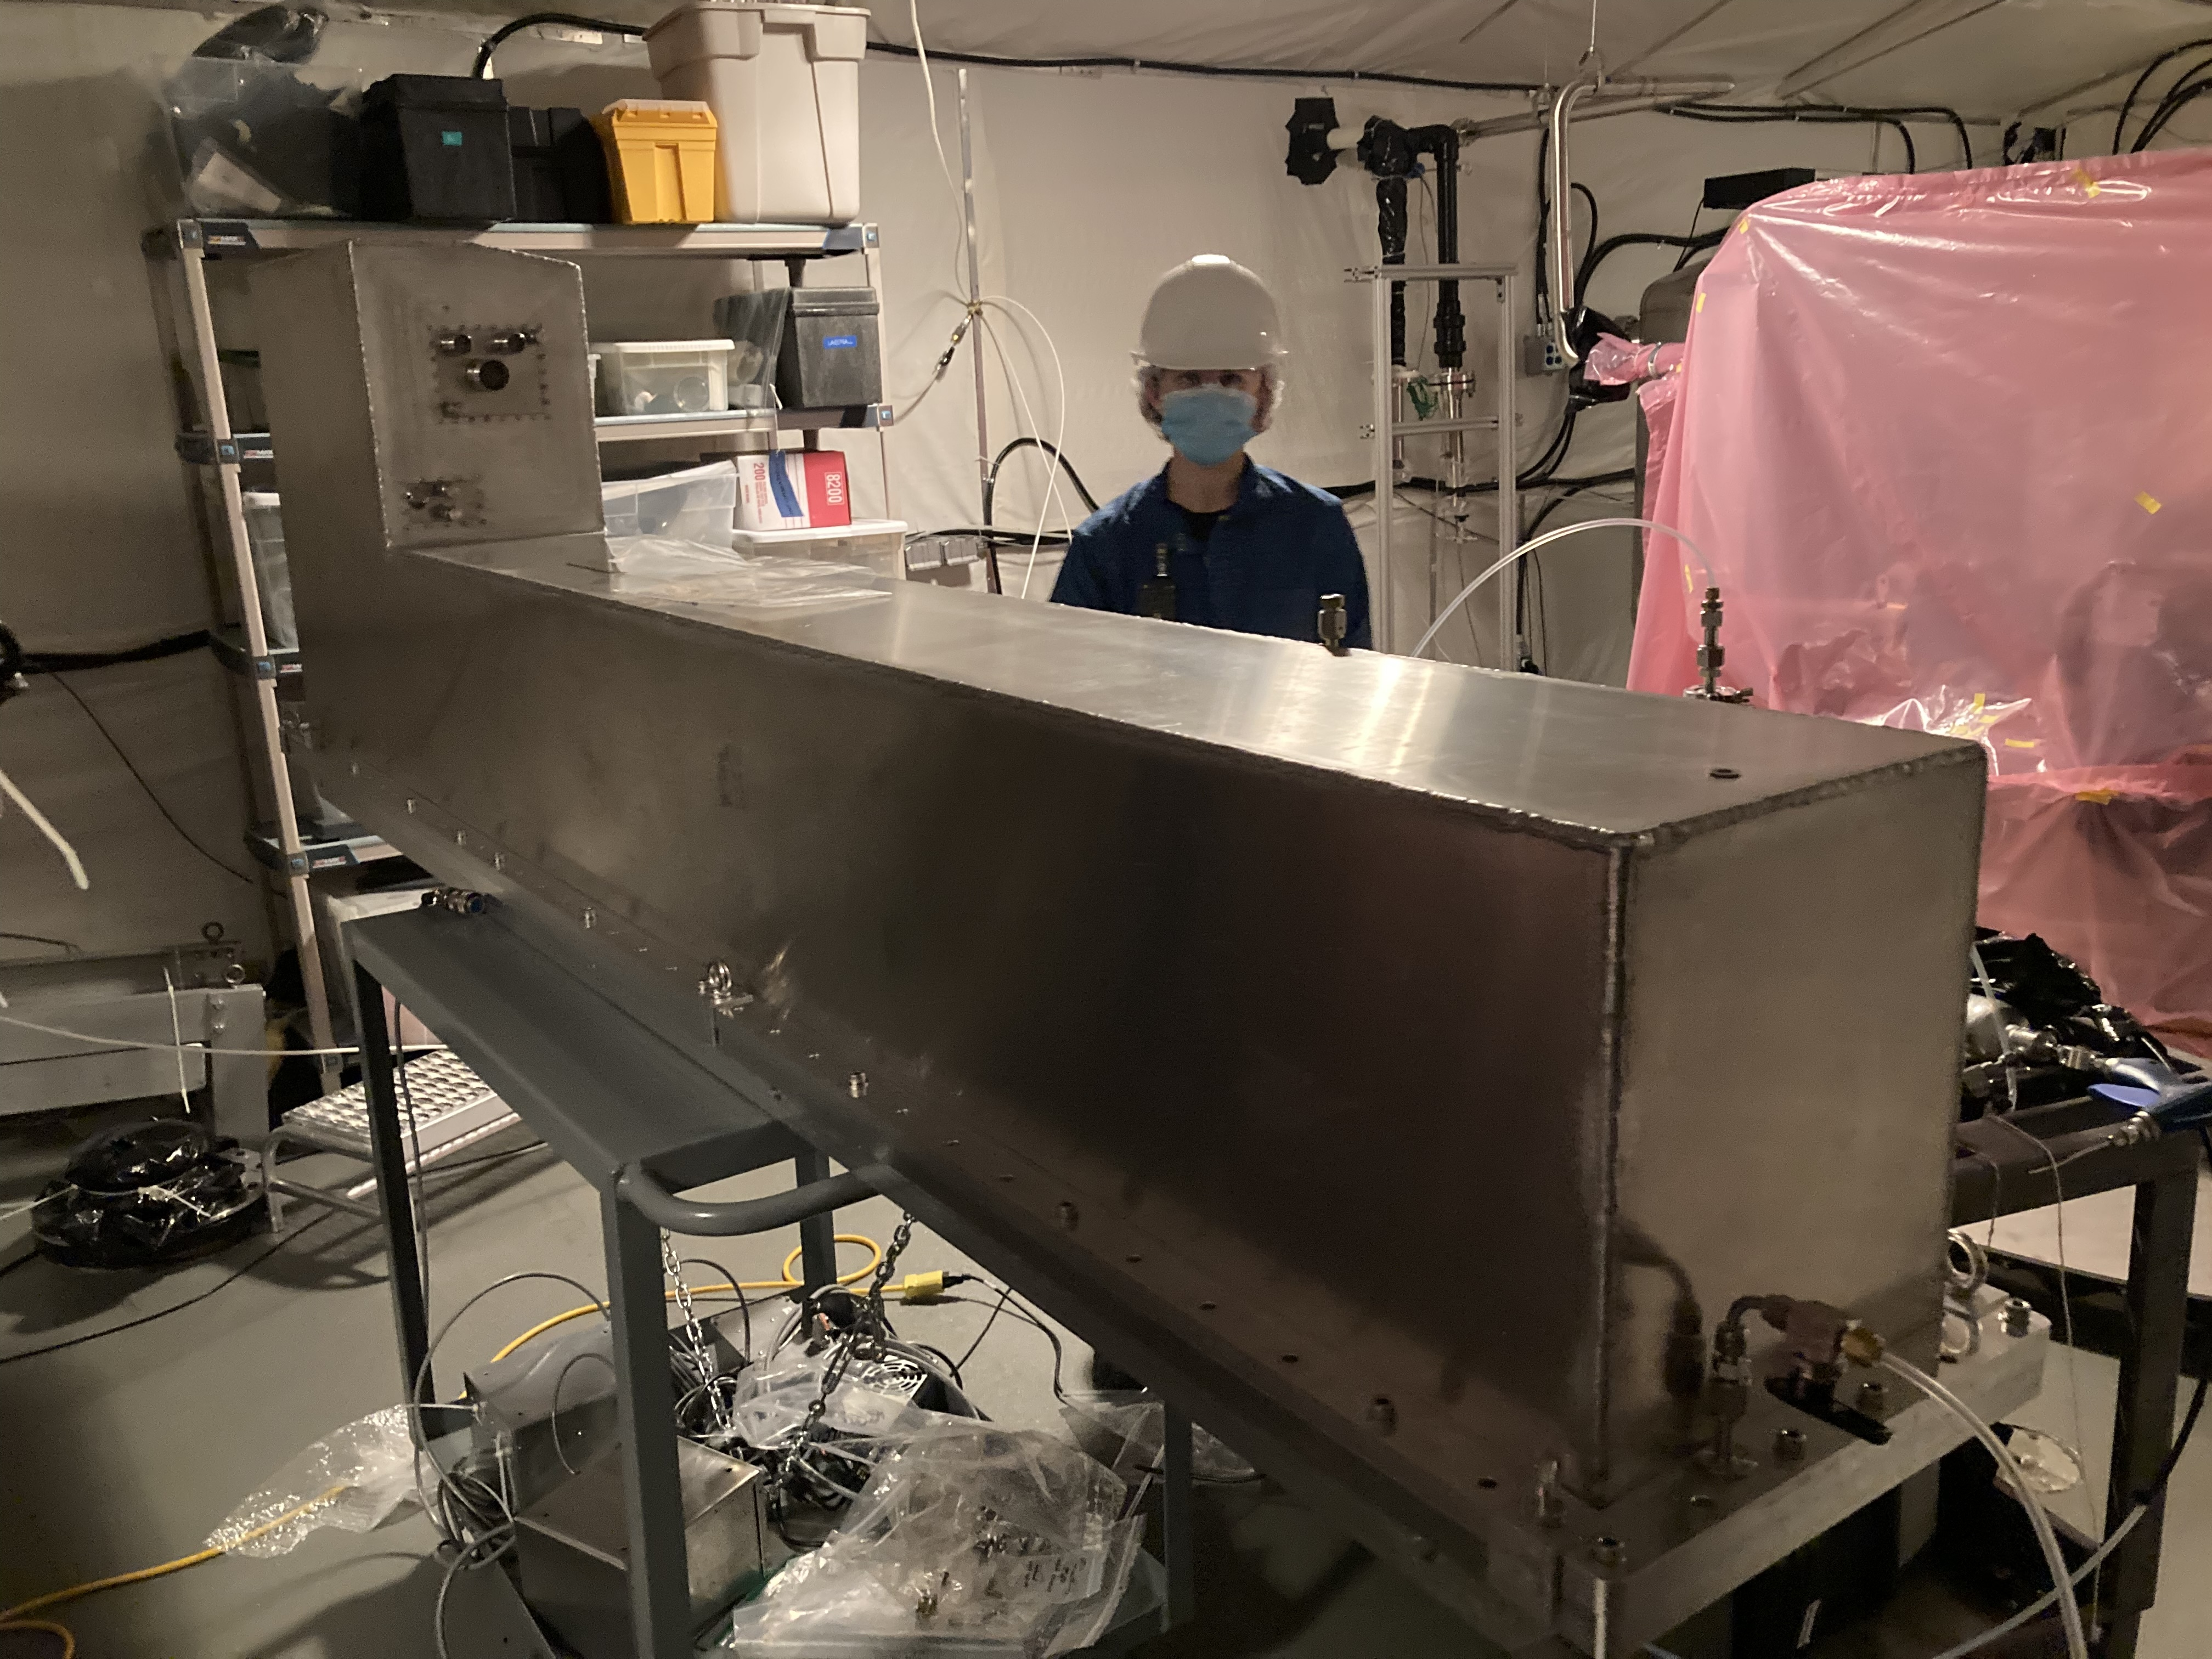
\includegraphics[width=0.7\textwidth]{Figures/20210712_190720132_iOS}
  \end{center}
  \caption{The Scintillator URM to be used for the source deployment}
  \label{fig:URM4}
\end{figure}

The following document describes the history of commissioning the URM at SNOLAB prior to describing how the URM must be prepared. This covers running the electrical subsystems checks, preparing the umbilical feed-through plate, the umbilical installation, the rope installation, the source connector installation, the cover installation, the source tube and bellows installation, the gatevalve installation, The final umbilical cleaning, the cover gas connection, and a test deployment procedure. The document concludes with a proposed order of operations and scheduling is shown at the end of the document.

\section{Definitions}
\begin{itemize}
\item AV: The acrylic vessel. A 12~m diameter acrylic sphere, fabricated for SNO, that currently contains the SNO+ scintillator cocktail.
\item PSUP: Photo-multiplier support structure. A geodesic sphere with an average diameter of 17~m, that supports the $\sim$9400 PMTs used to detect light in the SNO+ experiment.
\item Umbilical: a 1/2'' cable made by potting a HDPE tube surrounded by electrical wires inside a Tygothane tube using SilGel. The umbilical used here has a fibre optic bundle inside the HDPE core.  
\item Rope: 1/8'', white, braided, Tensylon fibre cord that has been shown to have good strength characteristics while being compatible with LAB. The central rope is installed on the URM while side ropes are made of the same material inside the AV. 
\item Calibration Source or Source: An item that can be deployed inside the scintillator volume that generates a known signal used to interpret the detector response. A dummy source will also be used which produces no signal, but will be used to test the manipulator system response.
\item URM: Umbilical retrieval mechanism. A device containing the umbilical and the central rope equipped with motors to deploy and retract both simultaneously and load cells to monitor the tension on the rope and umbilical. The umbilical is stored on a pair of pulley blocks connected to a charged piston that forces the blocks apart as the umbilical is retracted into the system. The rope is stored on a rotating drum.
\item UI: Universal interface. A 1.3 m diameter stainless steel vessel designed to contain a nitrogen cover gas over the SNO+ scintillator volume at the top of the AV neck. Equipped with a number of access points to deploy sensors, recirculate scintillator and deploy calibration sources.
\item DCR: Deck clean room. A tent on the SNO+ deck with additional HEPA filters to produce a clean environment for preparing calibration sources, or otherwise interaction with the AV interior. 
\item Source Bellows: A flexible stainless steel structure meant to connect the URM to the UI while allowing for the free movement of the UI. Must be terminated with a gatevalve. 
\item URM Hangers: Horizontal beams fixed to the DCR lifting beam. Includes rollers to allow for the limited use of lifting straps as well as turnbuckles to provide partial, semi-permanent support for the URM on rails
\item URM Lifting Table: table rated to lift 798 kg with an 80-20 paired frame with an interior hydraulic lifting system to raise the URM an additional 30~cm
\item URM Lifting System: Assembly of the URM hangers (specifically the lifting straps and winch) and the URM lifting table. It is essential that these be used in concert for stability when lifting the URM to height. 
\end{itemize}

\section{History}

\subsection{Arrival at SNOLAB, Cleaning and Testing, February 2017 - March 2019}
General comments about the handling: all operations with the URM were conducted in a cleanroom setting after the URM was placed in the SNOLAB cleanrooms and it was not removed from the cleanroom until after it was disassembled and bagged prior to being shipped underground. General guidelines were that the URM was never handled without cleanroom gloves on the hands of the workers and that the URM was cleaned after every interaction with UPW and Kimwipes. 
\begin{itemize}
\item {\bf June - August, 2017} URM completely disassembled, cleaned and reassembled. All large pieces were completely wiped with UPW. Screws were ultrasonically cleaned. 
\item {\bf August - September, 2017} Electrical systems and wiring for motors and sensors setup. Installed a rope to facilitate slipping and stretching measurements.
\item {\bf November 2017} Installed umbilical \#5 on URM after wiping down umbilical and URM with kim wipes and UPW (there was dust observed on the Umbilical).
\item {\bf June - August, 2018} Rope stretch tests in air, UPW and LAB. The contaminated rope was removed and never retracted into the URM.
\item {\bf August, 2018} Umbilical tests including running rope and umbilical together and umbilical slip tests (the umbilical did not slip under tensions up to 200 N).
\item {\bf September, 2018} Leak checked internal gas distribution systems to exclude leak rates above 10$^{-8}$ mbar L/s.
\item {\bf November 2018} Expanded the hole in the retraction pulley to accept an M4 eye-bolt.
\item {\bf January - September 2019} Redo rope stretch tests in air. 
\item {\bf September 2019} Installed limit switches at either end of
  the URM track.
\end{itemize}

\subsection{Transport Underground, January 2020}
See Cindy Lin's document on the preparation of the URM and conclusion of the transport underground, DocDB \href{https://www.snolab.ca/snoplus/private/DocDB/0061/006139/002/URM4_Final_Packing__Transporting_UG__and_DCR_Cleaning.pdf}{6139}. The summary is that the URM was disassembled, and all components were triple bagged before being crated up for transport underground. Once underground, the bags were systematically wiped down and removed starting with the outer layer in the outer car-wash, and the middle layer in the inner car wash before storage in the DCR. 

\subsection{Commissioning Underground to Date, May 2021 - August 2021}
\begin{itemize}
\item {\bf May 2021} Reassembled URM inside DCR. Surface cleaned parts by hand with Kimwipes and UPW. Some minor test of the electrical systems and reviewed the changes made to the limit switches.
\item {\bf July - September 2021} Leak check internal gas distribution components and cover flange. Installed externally flanged VCR ports and vents with gaskets.
\end{itemize}

\section{Remaining Procedures}

\subsection{Order of Operations}

The following procedures are described in by order of association, and not the practical order. To in fact assemble and commission the URM the processes should be done in the following order. 
\begin{answerlist}
\item Preparation of umbilical feed-through plate; Sec.\ref{ss:umbPrepFeed} (1 shift, machine shop?)
\item Remove URM cover; Sec.\ref{ss:rmCov} (1 shift, 4 workers)
\item Electrical systems check; Sec.\ref{ss:elecSSC} (1 shift, 1 worker)
\item Clean the umbilical; Sec.\ref{ss:cleanUmb}
\item Clean the surfaces of the pulley blocks and drive pulleys; Sec.\ref{ss:cleanURM}
\item Install umbilical on URM; Sec.\ref{ss:UmbInstall} (1 shift, 3 workers)
\item Install umbilical feed-through plate on umbilical; Sec.\ref{ss:umbPrepFeed} (1 shift, 2 workers)
\item Install rope on URM; Sec. \ref{ss:RopeInstall} (1 shift, 2 workers)
\item Install URM cover; Sec.\ref{ss:CoverInstall} (1 shift, 4 workers)
\item Transfer URM from cart to lifting table; Sec.\ref{ss:transfer} (1 shift, 6 workers)
\item Electrical systems check; Sec.\ref{ss:elecSSC} (1 shift, 1 worker)
\item Install source tee flange; Sec.\ref{ss:SourceTeeInstall} (1 shift, 2 workers)
\item Epoxy the fibre bundles at both ends of the umbilical;
% \item Install the wheels on the URM; 
\item Install source bellows; Sec.\ref{sss:BellowsInstall}
\item Install gate valve; Sec.\ref{sss:GateValveInstall}
\item Install source connector on umbilical; Sec.\ref{ss:SourceConn} (1 shift)
\item Purge the URM and connect to the cover gas system; Sec.\ref{ss:CGConnection}
\item Final Umbilical cleaning; Sec.\ref{ss:UmbClean} (1 week)
\item Connect and clean the AmBe source (?) (1 week, 3 workers)
\item Connect URM to UI; Sec.\ref{ss:CGConnection} (1 shift, 3 workers)
\item Field test the manipulator system.; Sec.\ref{ss:Testing} (1 shift, 3 workers)
\end{answerlist}
The listed time and personnel requirements are estimates to within the nearest shift. Many of these tasks and procedures may take fractions of shifts, but there are few procedures that can be done in parallel; primarily tasks that affect completely different aspects of the URM without overlap.

\subsection{General Comments}
For all of the following procedures workers must keep the following points in mind.
\begin{itemize}
\item Workers must use proper PPE for working in the underground clean lab
\item All procedures are to be conducted in the DCR.
\item Assume that nitrile clean room gloves are to be worn at all times.
\item When working on the interior workings of the URM
  \begin{itemize}
  \item Double gloves must be worn. Inside and outside gloves should be rinsed with UPW after they are donned.
  \item After handling lubricants or oils, the outer gloves must be removed and replaced.
  \end{itemize}
\item Every effort must be made to maintain the integrity and cleanliness of the DCR.
\item When the inner workings of the URM are exposed to the DCR, the dust counts should be monitored. Prior to work beginning, the number of 0.5$\mu$m particles must be less than 200 per cubic foot.
\item Workers must change coveralls if they work in specific locations prior to conducting work in the DCR including the underground machine shop and the inner car-wash.
\item Workers must shower and change clothes if they work in specific locations prior to working in the DCR including the scintillator plant and the outer car-wash. 
\end{itemize}

\subsection{Personal Protective Equipment: Donning Gloves}\label{ss:Rgloves}
The general glove cleanliness protocol requires that operators exercise extreme care when handling equipment that will come into contact with the detector scintillator.
\begin{answerlist}
\item Thoroughly wash and dry hands.
\item Put on a pair of clean room nitrile gloves.
\item Spray with UPW and rub hands together.
\item Rinse with UPW.
\item Dry with Kimwipe.
\item Put another pair of clean room nitrile gloves.
\item Spray UPW on the clean room gloves and rub hands together.
\item Rinse with UPW.
\item Dry with Kimwipe.
\end{answerlist}


\subsection{Removing the URM Cover}\label{ss:rmCov}
The first step to the majority of the activities to commission the URM is to remove the cover. The URM has been stored with the cover on to protect it from dust contamination. 
\begin{answerlist}
\item Remove the screws from the electrical and umbilical feed-through plates. Carefully remove the feed-through plates from the URM cover.
\item With an M6 hex and crescent wrench, remove the bolts holding the URM cover flange to the base. Store the nuts, bolts and washers so that they can be easily found and used. 
\item Ensure that the support feet and eye-bolts are secured to the flange at the four corners of the URM cover.
\item Prepare an area out of the way of other activities to place the URM with a piece of plastic suitable to be wrapped over the URM cover.
\item With four workers; one at each corner; with an appropriate height assist, lift the URM cover straight up off of the URM flange until it is clear of the URM backplane.
\item Carefully lower the URM cover onto the prepared plastic sheet. Wrap the sheet over the URM cover.. 
\item Check the URM o-ring. Ensure that it remains in its groove with no obvious damage.
\item Install the bumpers on the URM flange to protect both the URM flange surface and the o-ring using the same bolts as those that secured the cover to the base. 
\end{answerlist}

\subsection{Electrical Subsystems Check}\label{ss:elecSSC}
It is essential that the electrical systems be checked periodically
through this procedure to ensure that there is no loss of
function. The 20 pin feed-through is somewhat fragile and is easily
put under strain when the cover is removed or replaced. Tests must be
conducted with a manipulator control unit, and URM power
supplies. Tests should be conducted with the URM cover removed.

Running the electrical system requires
\begin{itemize}
\item A Special paired cable connecting to a single 20 pin Amphenol connector at one end and a pair of DB-15 bus connectors on the others
\item A AVR control box shown in fig. \ref{fig:AVRUnit}
\item Two Motor power supply boxes; each must have a power cable and a 6 pin Amphenol connector terminated output cable integrated into the box.
\item Two four pin motor control cables
\item One AVR power supply
\item An extension sufficient to reach the Manip computer in the DCR garage
\item The URM with the cover off.
\end{itemize}

\begin{figure}
  \begin{center}
    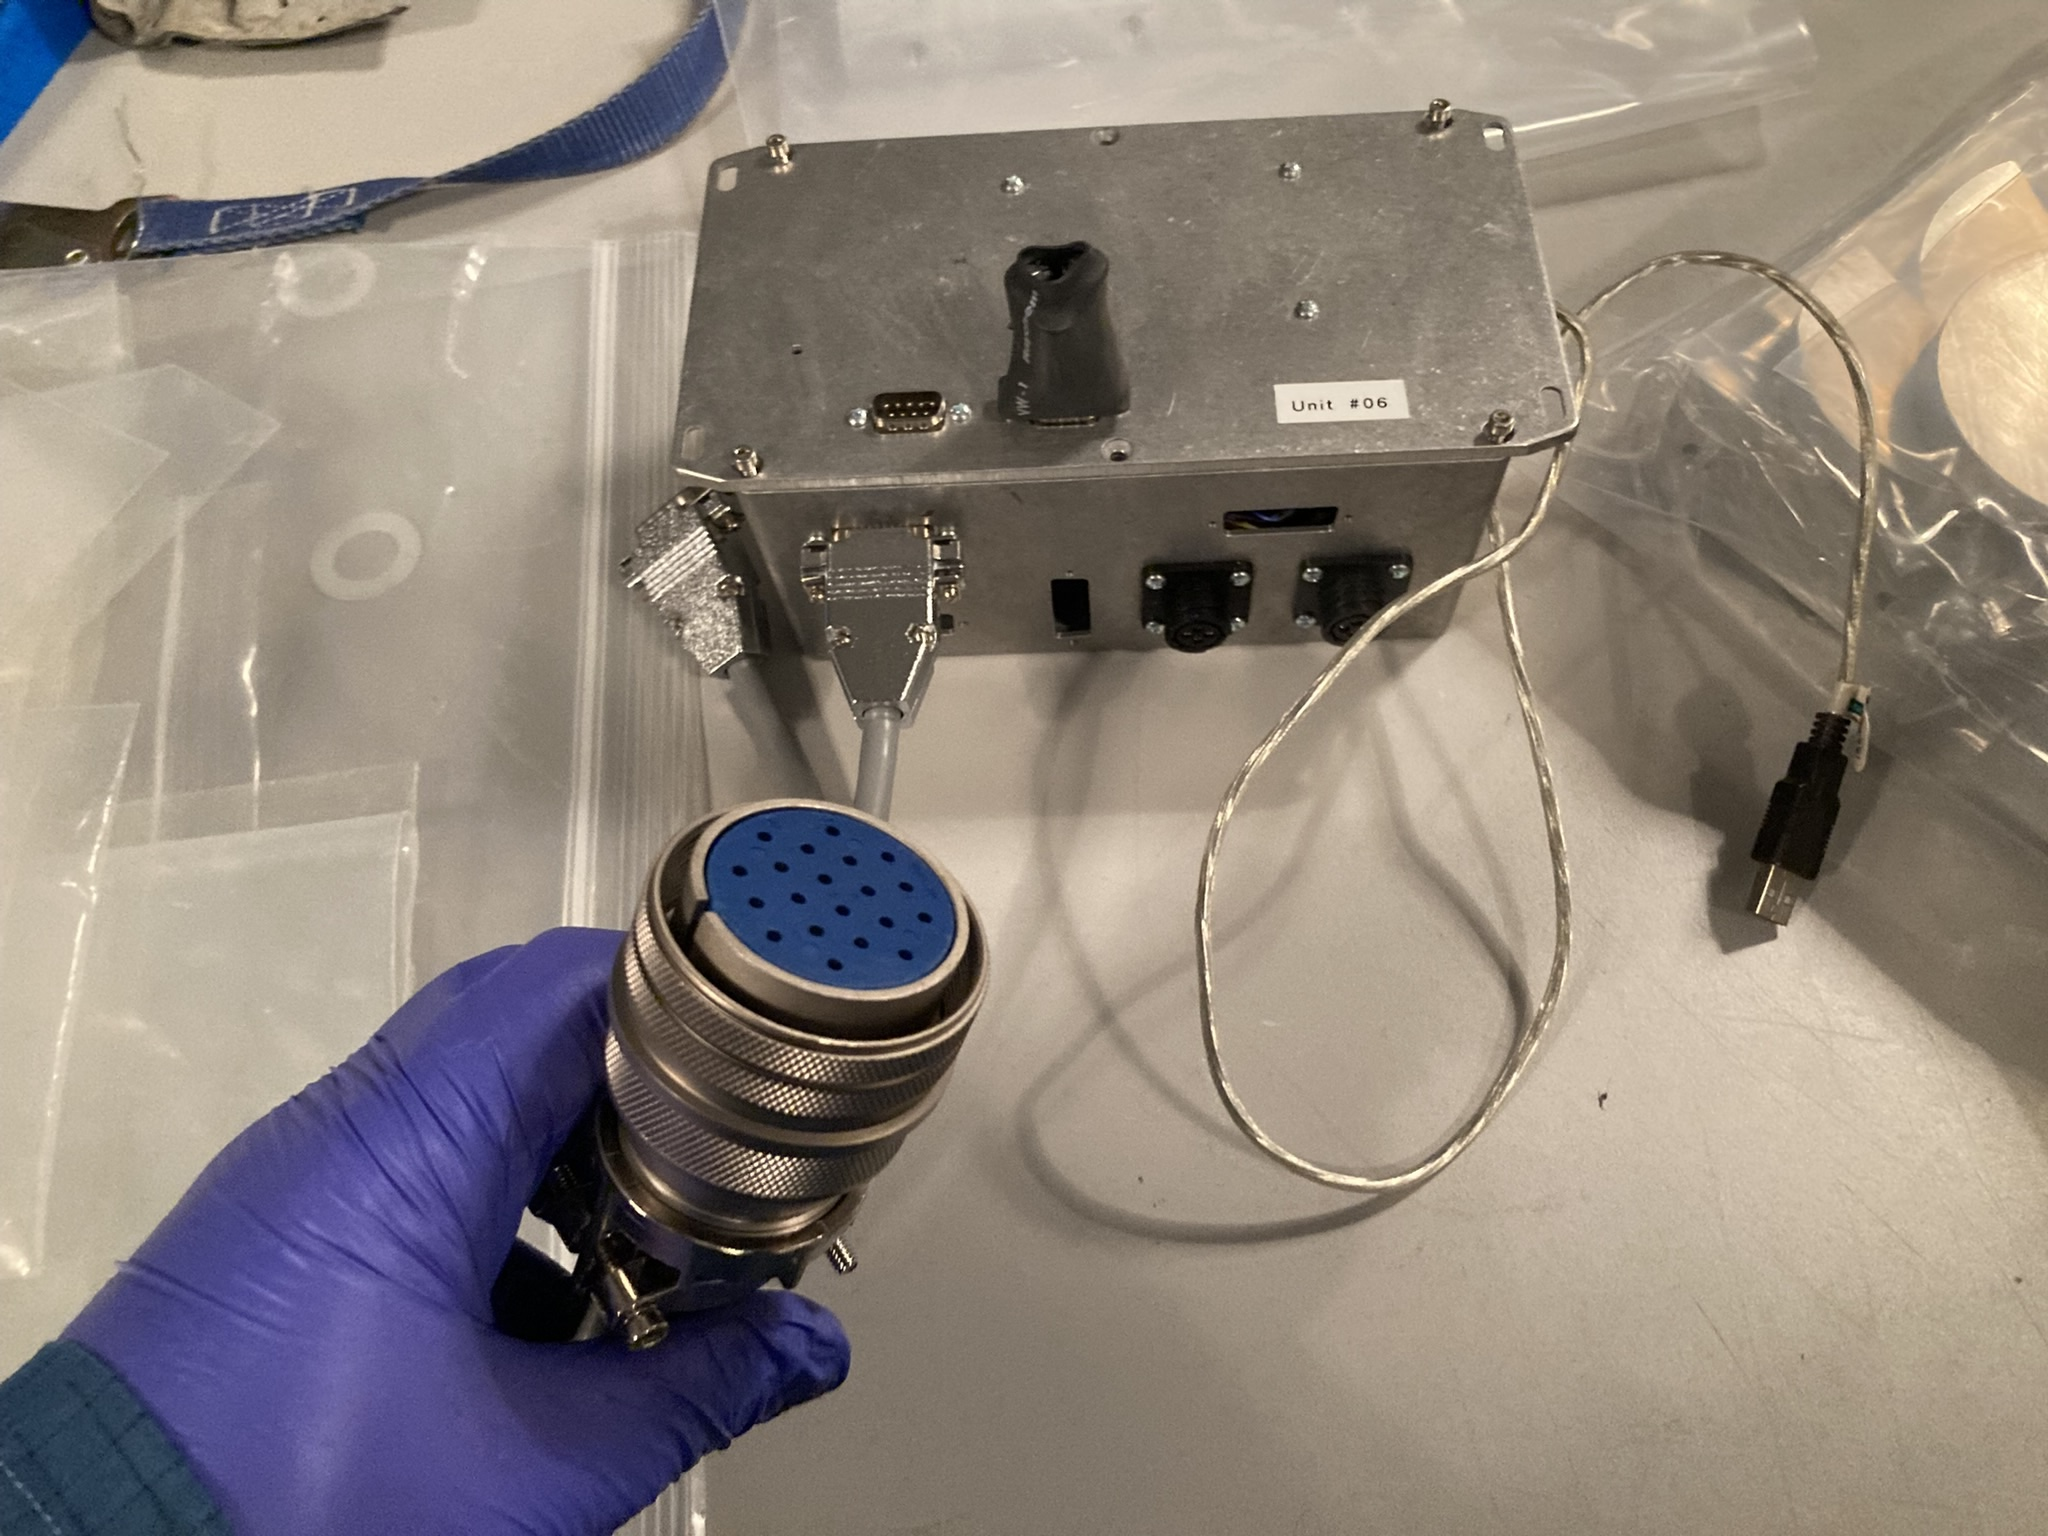
\includegraphics[width=0.6\textwidth]{AVRBox}
  \end{center}
  \caption{The box containing the AVR controller boards that are to be used with URM4}
  \label{fig:AVRUnit}
\end{figure}
  
  
\begin{enumerate}[label={$\square$}]
\item Connect the components as shown in Fig. \ref{fig:controller}.
  \begin{itemize}[label={$\square$}]
  \item The Rope and Umbilical sense cables attach to the URM via the
    20 pin socket mounted to the electrical feed-through plate,
  \item the DB-15 ends of the Rope and Umbilical sense cables connect
    to the AVR Unit via the appropriate socket. Convention has the
    Umbilical on the bottom and the rope on the top connector, but
    this should be verified with the Manip configuration on the
    Calibration Computer.
  \item The 6 pin Amphenol terminated control cables connect to 6 pin
    sockets, when looking at the feed-through plate from the outside,
    the umbilical motor control cable should be connected to the right
    feed-through socket and the rope connected to the left feed-through
    socket.
  \item The two four pin motor control cables run between the AVR
    control unit and the the motor power supply units.
  \item Connect the USB cable to the Manip computer USB extension,
    usually kept on the Northwest side of the UI.
  \item Plug the motor power supplies and the AVR power supply into an
    extension cable. Ensure that the fan is running on the AVR power
    supply. Make sure that the power switches on the motor supplies
    are set to on and the red LED lights are illuminated.
  \item Connect the AVR box to the computer power supply via the bus
    cable connector on the top of the AVR box. Ensure that the fan
    still runs after connecting the power supply and that the green
    LED light inside the AVR box is illuminated.
  \end{itemize}
\item Go to the Calibration computer and check if the appropriate AVR board
  is connected.
  \begin{itemize}[label=$\square$]
  \item Open a terminal and navigate to the \verb+AVR32+ directory
  \item Run the command \verb+manip+
  \item At the \verb+manip+ command prompt run \verb+init+
  \item Check the list of connected AVRs. Ensure that the AVR connected to URM4 appears in the list.
  \item Run the command \verb+show laserball+ on the command prompt. Disconnect URM2rope and URM2umbilical from the Laserball using the \verb+laserball disconnect+ command if necessary.
  \item In manip, connect the URM4rope and URM4umbilical objects to
    the Laserball source and check if the URM is receiving feedback on
    the load cells. If not the system will need to be debugged,
    starting with ensuring that the correct AVR connects to the the
    URM4rope and URM4umbilical objects in the \verb+WIRING.dat+ file
    in the \verb+AVR32+ directory
  \item Run the rope and umbilical by running the motors directly from
    the manip interface.
  \item Test the limit switches by moving the retraction block to either
    end of the track. If the limit switch signals are not detected by
    the manip interface, the reason must be understood and corrected.
  \end{itemize}
\end{enumerate}

\begin{figure}
  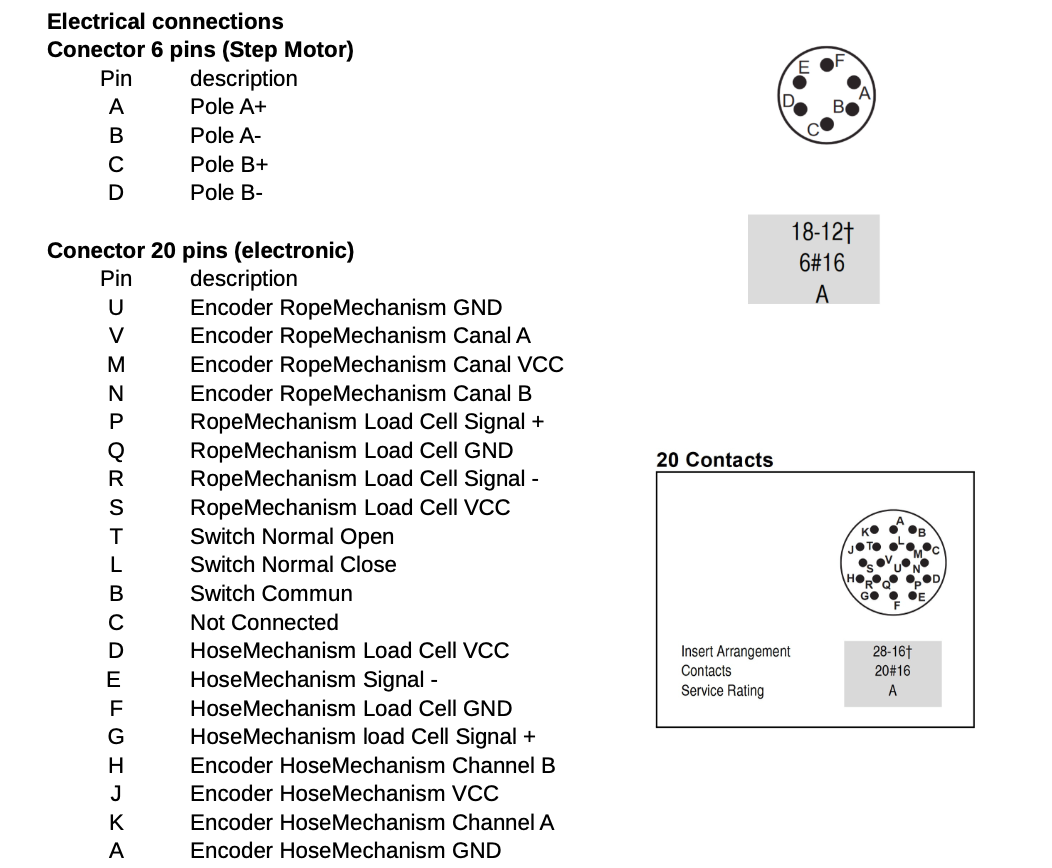
\includegraphics[width=0.8\textwidth]{20ConnectorPinOut}
  \caption{Pin out diagram for the URM as of August 2017. One minor revision made to incorporate the limit switch circuits in 2021.}
  \label{fig:pinout}
\end{figure}

\begin{figure}
  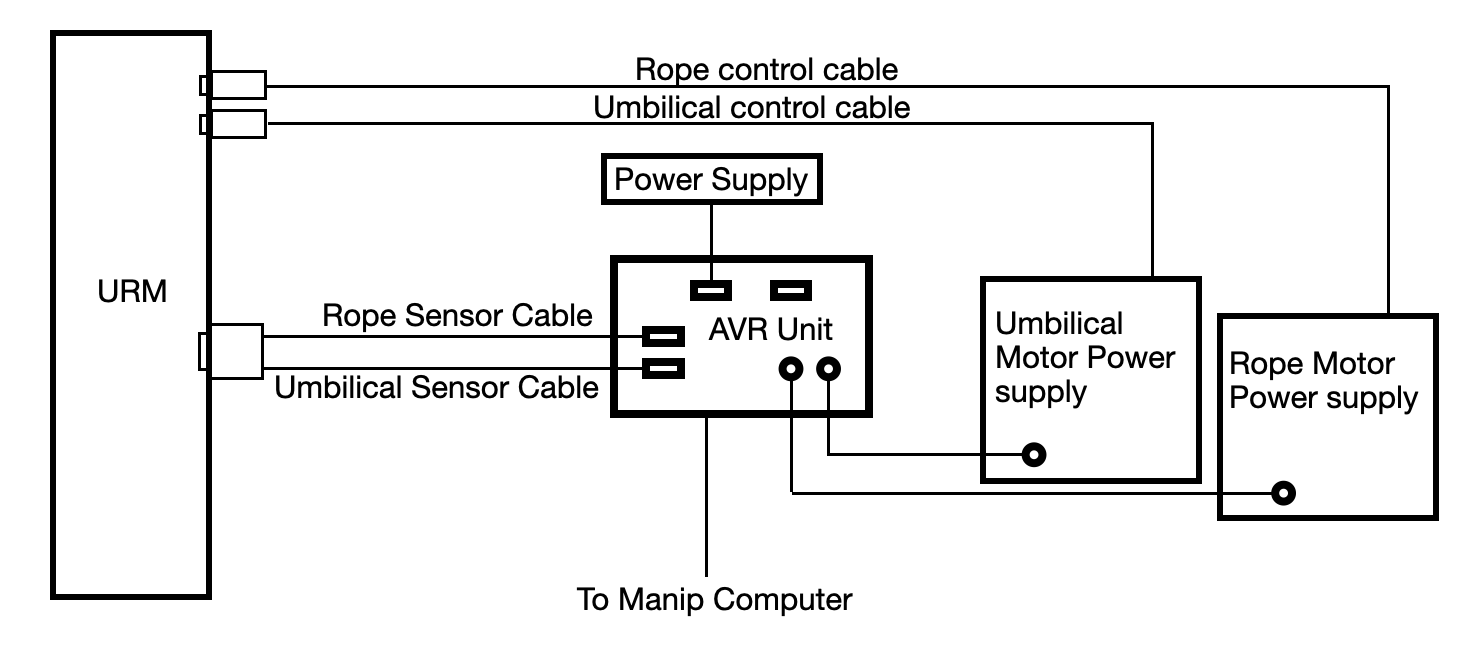
\includegraphics[width=\textwidth]{URMAVR_Setup}
  \caption{Diagram of AVR controller setup for URM.}
  \label{fig:controller}
\end{figure}

\subsection{Cleaning the Umbilical}\label{ss:cleanUmb}
The umbilical to be used is the 8th scintillator umbilical assembled
at Queen's in 2016. This is the only umbilical synthesized with a
fiber optical bundle. The umbilical was wiped once with acetone, then
with methanol in the Queen's clean lab and stored in a clean bag
inside of a nitrogen filled mylar bag. From 2017 to 2024 the umbilical
in its bag in the bottom of a cabinet in SNOLAB cleanroom A. It was
moved from the cleanroom as the Diol still commissioning ramped up and
is sitting on a desk with two additional plastic bags over the mylar
bag. Prior to further installing the umbilical on the URM, the
umbilical must be cleaned. For this procedure it is assumed that the
following materials are on hand in the DCR
\begin{itemize}
\item The umbilical in its original mylar bag
\item A spill tray suitable to catch LAB
\item A supply of clean LAB
\item A supply of UPW
\item Nitrile, clean-room gloves
\item poly gloves 
\item fisher-brand, Poly-cellulose cleanroom wipes (should start with an unopened pack)
\item Two clean plastic bag suitable made from pink static resistant plastic (inside the DCR).
\item A heat sealer
\item A nitrogen source (using a standard bottle on deck) with a regulator and a flow meter.
\end{itemize}
Cleaning the umbilical is to be done in a two step process. This
should be done between three workers; two to handle the umbilical and
one to provide additional help or go for additional items if needed. The first step provides an initial starting point for the cleanliness of the umbilical, while the second step prepares the umbilical for loading on the URM. To initially clean and evaluate the state of the umbilical
\begin{answerlist}
\item Prepare a spill tray by wiping it out with UPW and lint free
  cloths. Similarly clean the beige working tray and put it to one
  side.
\item Don clean-room gloves using the procedure in section \ref{ss:Rgloves}
\item Open the top of the umbilical storage bag. 
\item With one worker holding the bag, pull the umbilical from the bag
  and place it in one corner of the spill tray.
\item Ispsect the outside of the umbilical for damage.
\item Pick out one end of the umbilical. Shine a light into the one
  end of the umbilical and look for the light at the other end. The
  light should be visible at the ends of the fibers on the opposite
  end, even though the bundle is not yet complete. Count and record
  the illuminated fibers.
\item Designate one end of the umbilical as the standing end. This
  will be the end of the umbilical that will be secured to the URM
  umbilical feed-through. Both the standing end and the running end of
  the umbilical (the end to which the source will be connected) are
  identical and the fibre bundles will need to be terminated after
  loading onto the URM (the procedure of which will be communicated
  elsewhere).
\item Protect the ends of the umbilical. This can be done by wrapping
  the end in plastic wrap, or a plastic sleeve held in place with a
  zip tie. It is expected that the ends of the fibers are flush with
  the ends of the umbilical at this time, so this will mostly
  protect the fibers as they flex during installation. Cap the standing
  end of the umbilical with a different colour sleeve relative to the
  running end.
\item Wet a lint free cloth with UPW.
\item Starting with the running end, wipe the umbilical in strokes
  towards the standing end with UPW. Coil the umbilical in the
  opposite side of the spill tray. Be sure to keep an eye out for
  kinks and possible surface damage to the umbilical throughout this
  process.
\item Once the entire umbilical has been wiped down transfer the umbilical to a clean pink plastic bag.
\item Insert an open line to the nitrogen source into the bag with an outlet line. Seal the plastic bag with the heat sealer so the inlet and outlet lines are contained. Open the valve to the nitrogen supply with an output pressure on the order of 20 psi at a flow rate of 5 L/min. This will dry out the umbilical in a contained way. Leave the umbilical in this configuration overnight.
\item After drying the umbilical completely, open the bag and place the umbilical in the spill tray. Take tape lifts from various locations along the length of the umbilical and submit the tape lifts for XRF analysis. 
\item Return the umbilical to the plastic bag. Fill the bag with nitrogen and heat seal the bag.
\item Store the umbilical in a bin to protect the bag until use. 
\end{answerlist}
A second cleaning procedure should be followed immediately prior to loading the umbilical onto the URM; ideally in the same shift. Again this procedure should be completed by two workers with a third in reserve to handle 
The two workers must take the following 
\begin{answerlist}
\item Prepare a spill tray by wiping it out with UPW and lint free
  cloths. Similarly clean the beige working tray and put it to one
  side.
\item Don clean-room gloves using the procedure in section \ref{ss:Rgloves}
\item Open the top of the umbilical storage bag. 
\item With one worker holding the bag, a second should pull the
  umbilical from the bag and place it in one corner of the spill tray.
\item Inspect the umbilical again. Pick out one end of the
  umbilical. Shine a light into the one end of the umbilical and look
  for the light at the other end. The light should be visible at the
  ends of the fibers on the opposite end, even though the bundle is
  not yet complete. Count and record the illuminated fibers.
\item Wet a lint free cloth with clean LAB.
\item Identify the running and standing ends of the umbilical 
\item Protect the ends of the umbilical. This can be done by wrapping the end in plastic wrap, or a plastic sleeve held in place with a zip tie. It is expected that the ends of the fibers are flush with the ends of the umbilical at this time, so this will mostly protect the fibers as they flex during installation. 
\item Starting from the running end of the umbilical, wipe the
  Tygothane surface of the umbilical with the LAB wetted cloth with
  multiple passes on each section. Coil the umbilical loosely as you
  go in the opposite corner of the spill tray.
\item Once you get to the standing end of the umbilical, Store the
  cloth used to wipe the umbilical for particle counting analysis, and
  change outer gloves to use a new, clean pair.
\item Wet a new lint free cloth with clean LAB.
\item Flip the coil of umbilical over to access the running end again
  and, wipe the Tygothane surface of the umbilical with the LAB wetted
  cloth using multiple passes for each section. Coil the umbilical
  loosely in the corner of the spill tray opposite to that where it
  was coiled as you go.
\item Once complete, leave the standing end of the umbilical available
  for installation on the URM and cover the umbilical loosely with the
  beige spill tray. Store the outer gloves in a bag for appropriate
  disposal. Store the LAB wetted cloth for particle counting analysis.
\end{answerlist}

\subsection{Cleaning the URM (prior to umbilical installation)}\label{ss:cleanURM}
At each stage of the URM assembly, disassembly, movement underground and reassembly, the components of the URM have been cleaned with UPW and cleanroom wipes. The last opportunity to clean the URM before source deployment will be after the URM cover is removed and before the umbilical is installed. To clean the URM two workers will require
\begin{itemize}[label=$\square$]
\item a fresh supply of UPW
\item two spray bottles
\item a fresh pack of Fisherbrand, Poly-cellulose cleanroom wipes
\item supply of cleanroom gloves.
\end{itemize}
To clean the URM the workers must
\begin{enumerate}[label=$\square$]
\item Don clean room gloves using the procedure in section
  \ref{ss:Rgloves}.
\item Remove the front and rear pulley blocks, The umbilical motor
  assembly, the rope encoder pulley, and the sprung rope pulley.
\item Disassemble the front and rear pulley blocks, the rope encoder
  pulley, and the sprung rope pulley. Remove the guide and drive
  pulleys from the umbilical motor assembly. Submit the parts for
  ultra-sonic cleaning.
\item Clean the umbilical motor assembly with UPW and clean room
  wipes.
\item Reassemble the front and rear pulley blocks, the rope pulleys,
  and the pulleys on the motor assembly. N.B. URM5 is physically
  identical to URM4, so the pulleys and their support systems have
  already been cleaned ultrasonically, so the blocks, and rope pulleys
  can just be replaced. In contrast the umbilical motor assembly from
  URM5 was never tested, so the pulleys on the URM4 motor assembly
  should be replaced with the clean ones from URM5.
\item Mist the remaining surfaces of the URM and wipe the surface with
  the cleanroom wipes until the surface is again dry. This should
  include the URM backplane, support braces, bed, piston, and
  retraction pulley. Special care should be taken to wipe the bottom
  rope pulleys with UPW as it is extremely difficult to remove those
  pulleys from the system for ultrasonic cleaning without removing the
  back plane.
\item Wipe down the traveling pulley and bottom pulleys with UPW and
  clean room wipes. Use a standard swip test on the working surfaces
  of the pulleys to ensure that there is no evidence of grease
  remaining. If there is grease, clean the surface with isopropyl
  alchohol, before again cleaning with UPW and wipes.
\item Start the rope motor at low speed (50 rpm) to facilitate
  cleaning the rope drum. Use compact cotton swabs to get inside the
  rope groove on the rope drum and check to make sure that there is no
  residue on the swab it proceeds from the top of the groove to the
  bottom. If there is evidence of grease, wipe out the groove of the
  rope drum again with isopropyl alchohol and lint free wipes before a
  last pass with UPW and lint free wipes.
\item Replace the ultrasonically cleaned rope and umbilical pulley
  blocks. Replace the motor assembly with the cleaned pulleys
  installed.
\item Reconnect all of the system cabling (where necessary) and
  conduct a full electrical systems check.
\end{enumerate}

%The ideal way to secure the umbilical is very similar to how the
%umbilical is secured to the source; by using a set of pressure plates
%to provide an anchor point outside of the plate. The pressure plates
%should be pressed against the outside of the feed-through plate using
%bolts threaded into (currently non-exist ant) blind holes in the
%outside of the feed-through plate. Presuming that this altered
%feed-through plate exists the installation process consists of 
%\begin{answerlist}
%\item Put a clean cable tie around the umbilical at approximately the location of where the umbilical should nest against the inside of the feed-through plate
%\item Install a 1/2'' diameter o-ring on the umbilical and push it snugly against the cable tie
%\item Thread the umbilical through the feed-through plate such that the o-ring can be nestled against the in-ward facing side of the plate.
%\item Install a 1.2'' diameter o-ring on the umbilical and push it snugly against the outside of the feed-through plate.
%\item String a pressure plate onto the umbilical. Alternate an additional two 1/2'' diameter o-rings and pressure plates on the umbilical
%\item Put a little tension on the umbilical to press the inner o-ring against the inside of the feed-through plate.
%\item Push the pressure plates, one by one, against the outside of the pressure plate.
%\item Bolt the pressure plates to the outside of the feed-through plate.
%\item Allow the umbilical to relax. The o-rings between the pressure plates should grab onto the umbilical as it relaxes. Lightly test the holding power of the pressure plates by pulling on the umbilical from both sides.
%\end{answerlist}

\subsection{Umbilical Installation}\label{ss:UmbInstall}
This is a three person procedure; two workers handling the umbilical
and a third to run commands on the manip system. Both workers handling
the umbilical must wear clean nitrile gloves. The gloves should be
rinsed with UPW and dried before working. For the installation the
workers need
\begin{itemize}
\item to have the URM setup to run with commands from the manip system
\item the cleaned umbilical sitting loosely coiled in a spill tray
\item to ensure that the ends of the umbilical are protected, neatly, so that the ends of the umbilical will not catch on the 
\end{itemize}

\begin{answerlist}
\item If not already done, remove the cover over the umbilical exit port at the base of the URM. Replace the bolts afterwards to keep the interior reinforcing ring in place. 
\item Using a piece of Tensylon rope tie the retraction block at the
  end of the track to the piston in the closed position. A long piece
  of rope will be required for this as it will need to span the 1.2 m
  distance between the umbilical retraction block and the retraction
  pulleys munted to the pneumatic piston at least twice, so make sure
  that 3 m of rope is available when securing the system.
%\item Hang the umbilical feed-through plate from the bar supporting
%  the electrical feed-through. Also secure the umbilical to the URM
%  motor backplane.
\item With no pressure on the piston, push the retraction block as close to the fixed block as possible.
\item Start the URM motor at a constant 50 rpm. This should be with
  the supervision of a calibration expert first by executing the
  command \verb+avr3 m1 on 1+ followed by \verb+avr3 m1 dir 1+ and
  \verb+avr3 m1 ramp 50+. Ensure that the motor direction will retract
  the umbilical as it is fed through the system by checking the
  direction of the drive pulleys. One worker must monitor the system
  constantly and be in communication with the other workers who will
  be manipulating the umbilical, as there may be the need to start and
  stop the system at any time, or to otherwise change the motor rates
  when necessary.
\item Both umbilical workers should don gloves according to the
  procedure in section \ref{ss:Rgloves}.
\item Identify the standing end of the umbilical. Insert the umbilical
  into the exit port of the URM and carefully thread it between the
  first smooth guide pulley and the first toothed wheels of the motor
  mechanism. Be mindful of pinch points in the mechanism. Both workers
  will need to co-operate for this task as the gap between the toothed
  pulleys is held shut with a spring arm.
\item Continue to guide the umbilical end around the large toothed
  pulley and under the encoder pulley.
\item While one person continuing to guide the umbilical end over the
  remaining smooth guide pulley, the second will increase the motor
  revolution rate to 500 rpm.
\item Once the umbilical end is clear of the motor pulley system,
  start feeding the umbilical over the pulley in line with the motor
  system on the fixed block and the return block. Bend the umbilical
  over the return block with one worker guiding the umbilical end and
  one to collect the umbilical end on below the block while protecting
  the running end.
\item Continue guiding the standing end of the umbilical under the
  first pulley of the fixed block. Between two workers, bend the
  umbilical up and over the first pulley on the block. Continue
  guiding the umbilical over the second pulley of the return block and
  under the second pulley of the fixed block. Continue through the
  third, fourth, fifth and sixth pulley pairs.
\item After bending the umbilical under the sixth pulley of the fixed
  block allow the motor to run long enough to provide an additional 3.5
  meters of umbilical. Then stop the motor. The umbilical feed-through
  plate may now be installed on the standing end of the umbilical 3
  meters from the end. The 7.075 m of umbilical currently on the URM
  and the additional 4 meters above that will never exit the URM after
  installation is complete.
\item Connect a nitrogen gas bottle to the gas port at the bottom of
  the URM that connects to the piston at the motor box end through a
  pressure regulator and a ball valve. Set the regulator to output a
  pressure between 45 and 60 psi.  Ensure that the bottle internal
  pressure is greater than 500 psi to start and replace it otherwise.
\item One worker must hold the standing end of the umbilical
  firmly. Apply pressure to the piston by opening the ball valve
  carefully.
\item One worker must hold the umbilical at the standing end. The
  second worker will return to the Calibration computer, reverse the
  URM4 motor direction, and start the motor running again at a rate of
  500 rpm. This will retract the umbilical onto the URM. Stop the
  umbilical once it the end is less than 1 meter below the base of the
  URM, but more than 30 cm while waiting for further steps.
\end{answerlist}

\subsubsection{The Required Umbilical Length and the Feed-through Location}
The minimum distance between the pulley blocks is 216 mm. The diameter
of the pulleys are 205 mm. With 6 coils, a minimum length of 6.46 m
will be stored on the URM blocks. The distance between the front block
and the main drive pulley is 295 mm and the diameter of the drive
pulley is also 205mm. Given that the drive pulley is 230 mm above the
bed of the URM and that the umbilical does not follow a direct path
through the guide and encoder pulleys, the minimum length of 7.303 m
will be contained in the URM when the umbilical is fully
deployed. These dimensions are depicted in
Fig.\ref{fig:URMSideview}.

The expected distance between the URM and the gate valve is 1.357 m,
based on Fig.\ref{fig:URMpreUI}, while the distance between the gate
valve and the bottom of the AV is 14.43 m (as determined from
measurements recorded by Peter Skensved in the ``Calibration Log Book
\#6'' contained in the DCR. This means that the total length of
umbilical required when the umbilical is deployed (ignoring the source
length) is 23.09 m. Therefore 7 m of surplus umbilical (given the
manufactured length of 30~m) are available available after
loading. The 23.09 m can be comfortably stored on the URM given that
when the blocks are at their maximum extent the URM can hold 29.2
m. The placement of the feed-through plate should be done so that
there is an additional length of at least 2 m on the end of the
umbilical to accommodate the consolidation of the fibre bundle and the
installation of the source; more is likely better as having a length
of 3~m (suggested) will allow the end of the umbilical to be
comfortably manipulated for the sealing of the fibre bundle ends while
5~m could allow the umbilical to reach the dye laser without the use
of an additional patch cable. The position of the umbilical ends is
dictated by the position of the feed-through plate. To consolidate the
fibers at the end going to the laser, at least 3 m will be required so
that the work can be done on a comfortable surface adjacent to the URM
cart, so three meters is given as the minimum length of umbilical that
should be outside of the URM. Any difference in distance between the
end of the umbilical and the laser must be made up with a fiber optic
patch cable.

\begin{figure}
  \begin{center}
    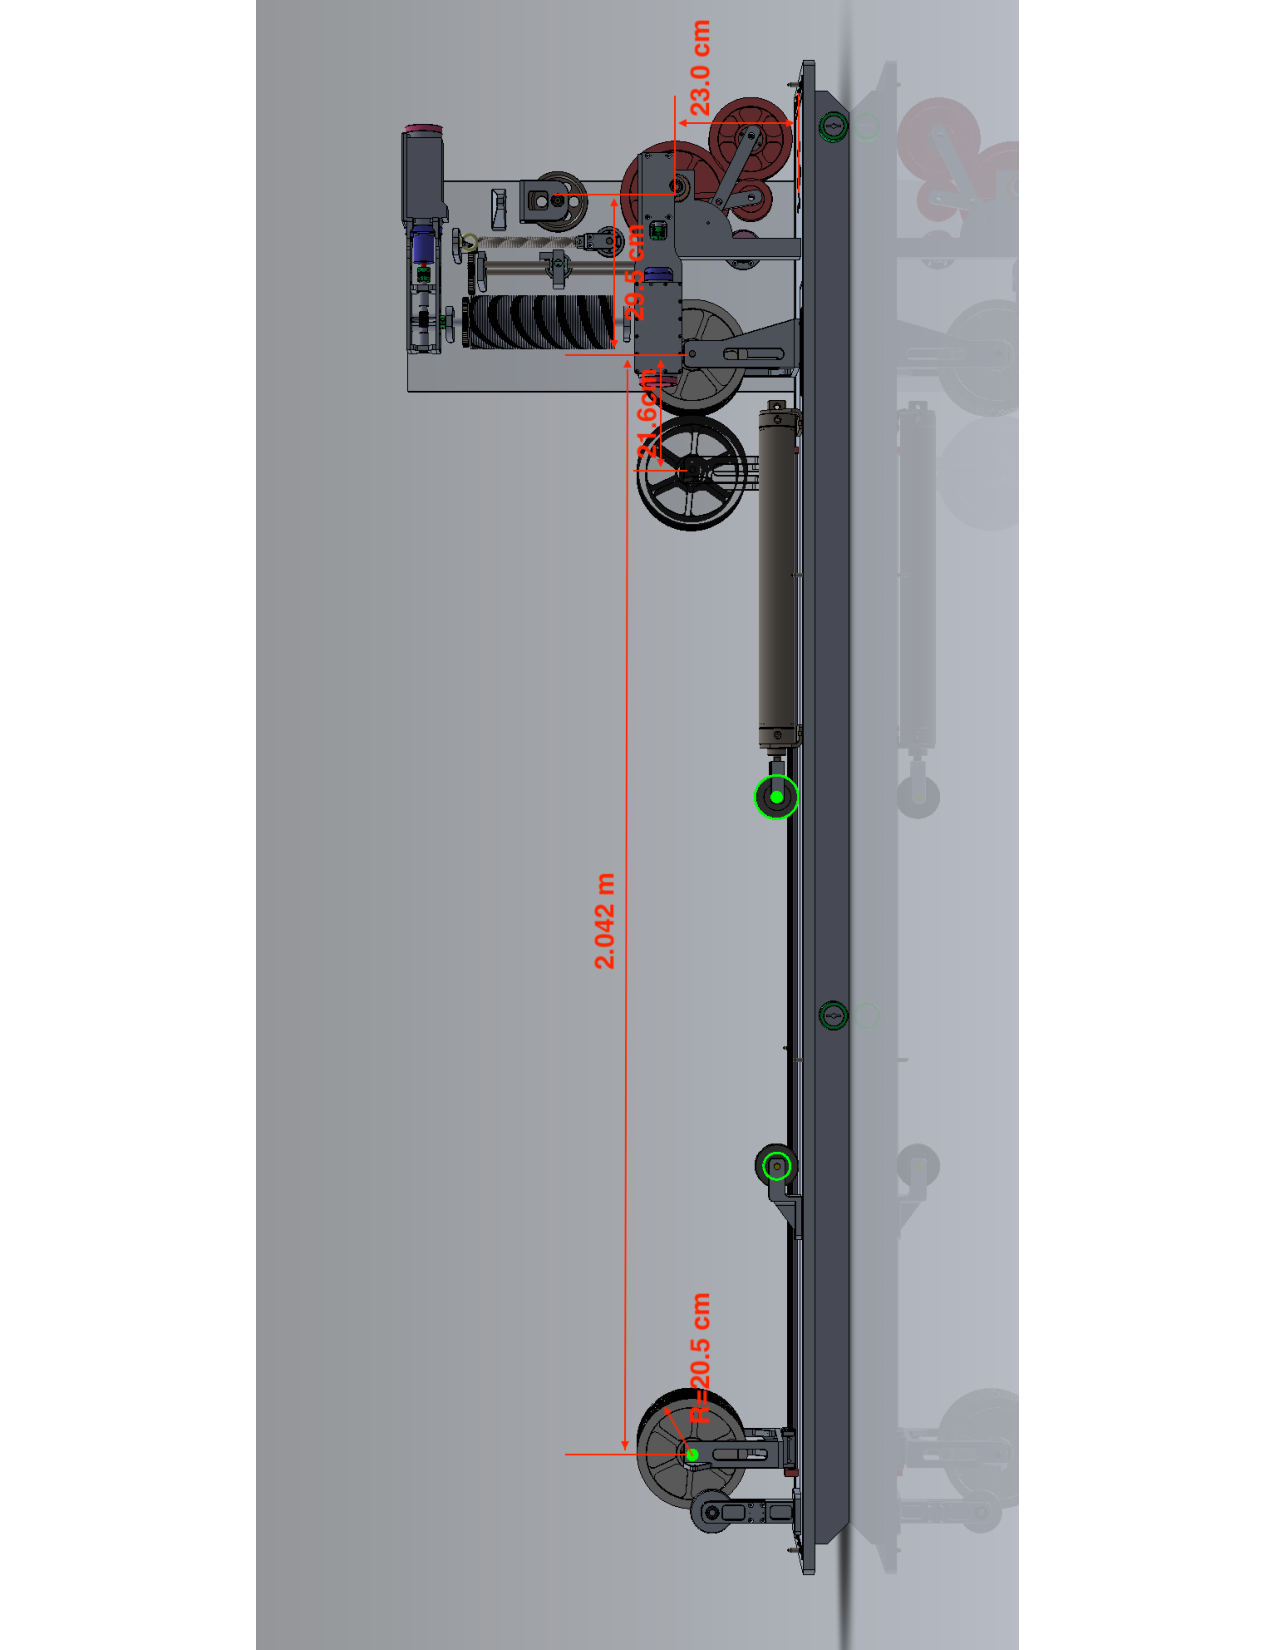
\includegraphics[height=\textwidth,angle=270]{URMSideview}
  \end{center}
  \caption{URM with the cover removed showing the minimum and maximum distance between the pulley blocks. The dimensions shown set the minimum and maximum umbilical lengths contained in the URM during deployment and after full retraction.}
  \label{fig:URMSideview}
\end{figure}

%The alternative procedure runs as follows.
%\begin{answerlist}
%item Using a piece of Tensylon rope tie the retraction block at the
%  end of the track to the piston in the closed position.
%\item Hang the umbilical feed-through plate from the bar supporting
%  the electrical feed-through. Also secure the umbilical to the URM
%  motor backplane.
% \item With no pressure on the piston, push the retraction block as close to the fixed block as possible.  
% \item Thread the umbilical through the bottom of the pulleys closest to the backplane (in the axis perpendicular to the back plane.
% \item Pass the umbilical over the top of the first return pulley and over the second pulley of the fixed block.
%\item Thread the umbilical under the second pulley of the fixed block back under the second pulley of the return block.
%\item Pass the umbilical over the top of the second return pulley and over the third pulley of the fixed block.
%\item Thread the umbilical under the third pulley of the fixed block back under the third pulley of the return block.
%\item Pass the umbilical over the top of the third return pulley and over the fourth pulley of the fixed block.
%\item Thread the umbilical under the fourth pulley of the fixed block back under the fourth pulley of the return block.
%\item Pass the umbilical over the top of the fourth return pulley and over the fourth pulley of the fixed block.
%\item Thread the umbilical under the fifth pulley of the fixed block back under the fifth pulley of the return block.
%\item Pass the umbilical over the top of the fifth return pulley.
%\item Place a clean container (spill tray or stainless steel pot) below the URM exit hole.
%\item Start the umbilical motor at 50 rpm
%\item Feed the umbilical under the leading, smooth pulley on the motor assembly, over the second smooth pulley. Then under the small, toothed encoder pulley and around the large toothed pulley to go between the bottom toothed pulley and the small, smooth guide pulley. Be mindful of pinch points as the motor must be running through this procedure.
%\item Once the path of the umbilical is set, allow it to continue running to pay the umbilical through the hole on the bottom of the URM. 
%\item Increase the rate to take up enough slack in the umbilical so that the umbilical is coiled firmly about the fixed and return blocks on the URM. Slow the motor when approaching that point and stop it completely before applying tension to the fixed end of the umbilical.
%\item Apply pressure to the umbilical piston between 40 and 50 PSI. The pressure should be applied slowly so that the rope is not shocked during the procedure
%\item Run the motor in the reverse direction to slowly load the umbilical onto the URM.
%\item Stop the motor with the last meter below the URM.
% \end{answerlist}


\subsection{Preparation of Umbilical Feed-through Plate}\label{ss:umbPrepFeed}

A dummy feed-through plate was provided with the URM that has a molded
central piece to suggest an umbilical port. It was not milled for an
umbilical however and there was no specific plan for securing the
umbilical to the URM. It is proposed here to use a Swagelok bulkhead
fitting to provide a seal against and strain-relief for the umbilical
itself. Incorporating telfon material between the bulkhead and the
plate at either end with washers and teflon tape through the run of
the threads should make this leak tight. To accommodate this the plate
should be milled through with a 3/4'' hole and threaded with a
3/4''-20 tap. This hole should be milled through the angled cap with
the edges milled down to allow a flat surface for the bulkhead nuts
(one of which is part of the bulkhead fitting) with space to connect
the backing nuts on the bulkhead.  Once the umbilical is fed through
the bulkhead fitting, it can be swaged to the umbilical on either side
with PTFE ferrules to provide a gas seal to the umbilical without
damaging the umbilical. A mockup of the umbilical feedthrough plate,
with the umbilical, is shown in Fig.\ref{fig:UmbilicalFeedthrough}.

\begin{figure}
  \begin{center}
    \begin{subfigure}{0.3\textwidth}
      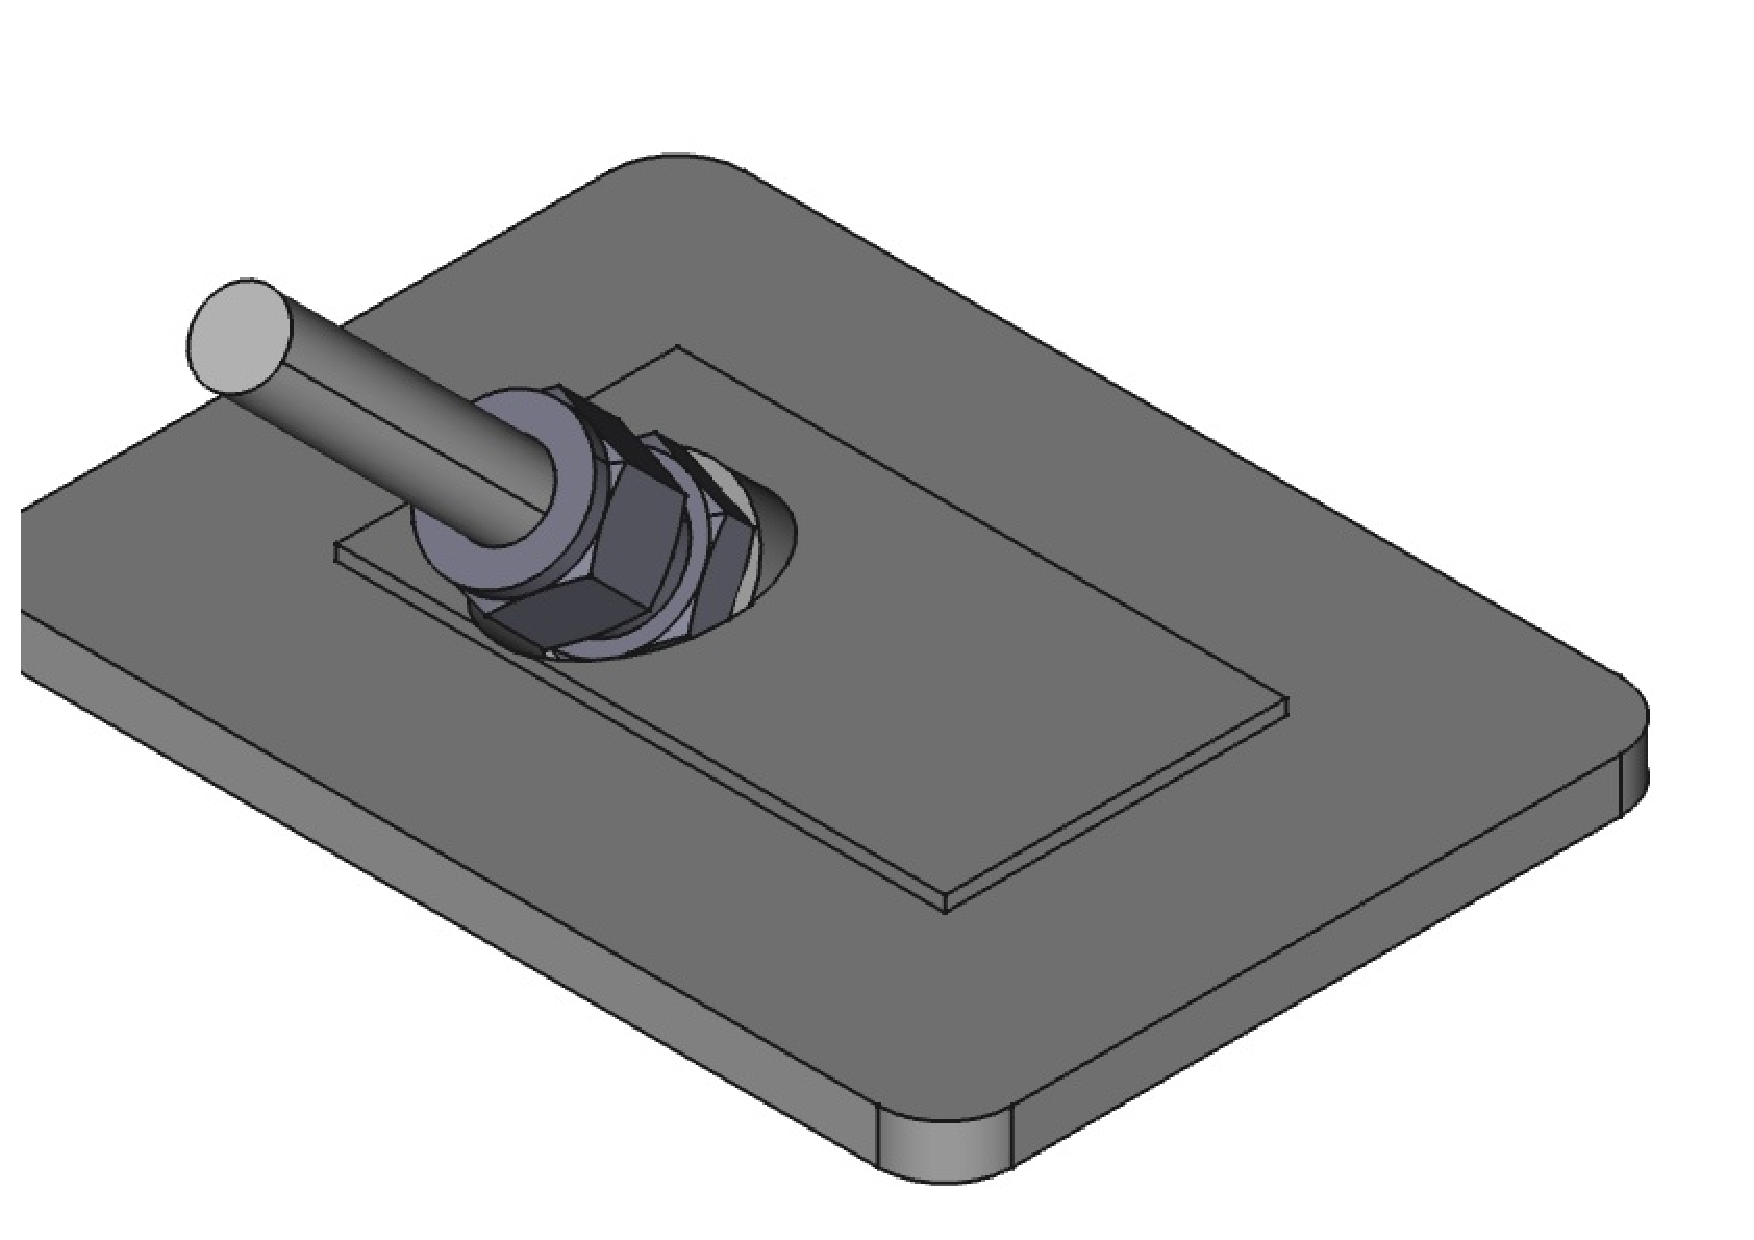
\includegraphics[width=\textwidth]{UmbilicalFeedthroughOrtho_2.pdf}
      \caption{Orthographic view of feedthrough plate}
      \label{fig:UFOrtho}
    \end{subfigure}
    \begin{subfigure}{0.3\textwidth}
      \includegraphics[width=\textwidth]{UmbilicalFeedthroughSideview_2.pdf}
      \caption{Sideview of feedthrough plate}
      \label{fig:UFSide}
    \end{subfigure}
    \begin{subfigure}{0.6\textwidth}
      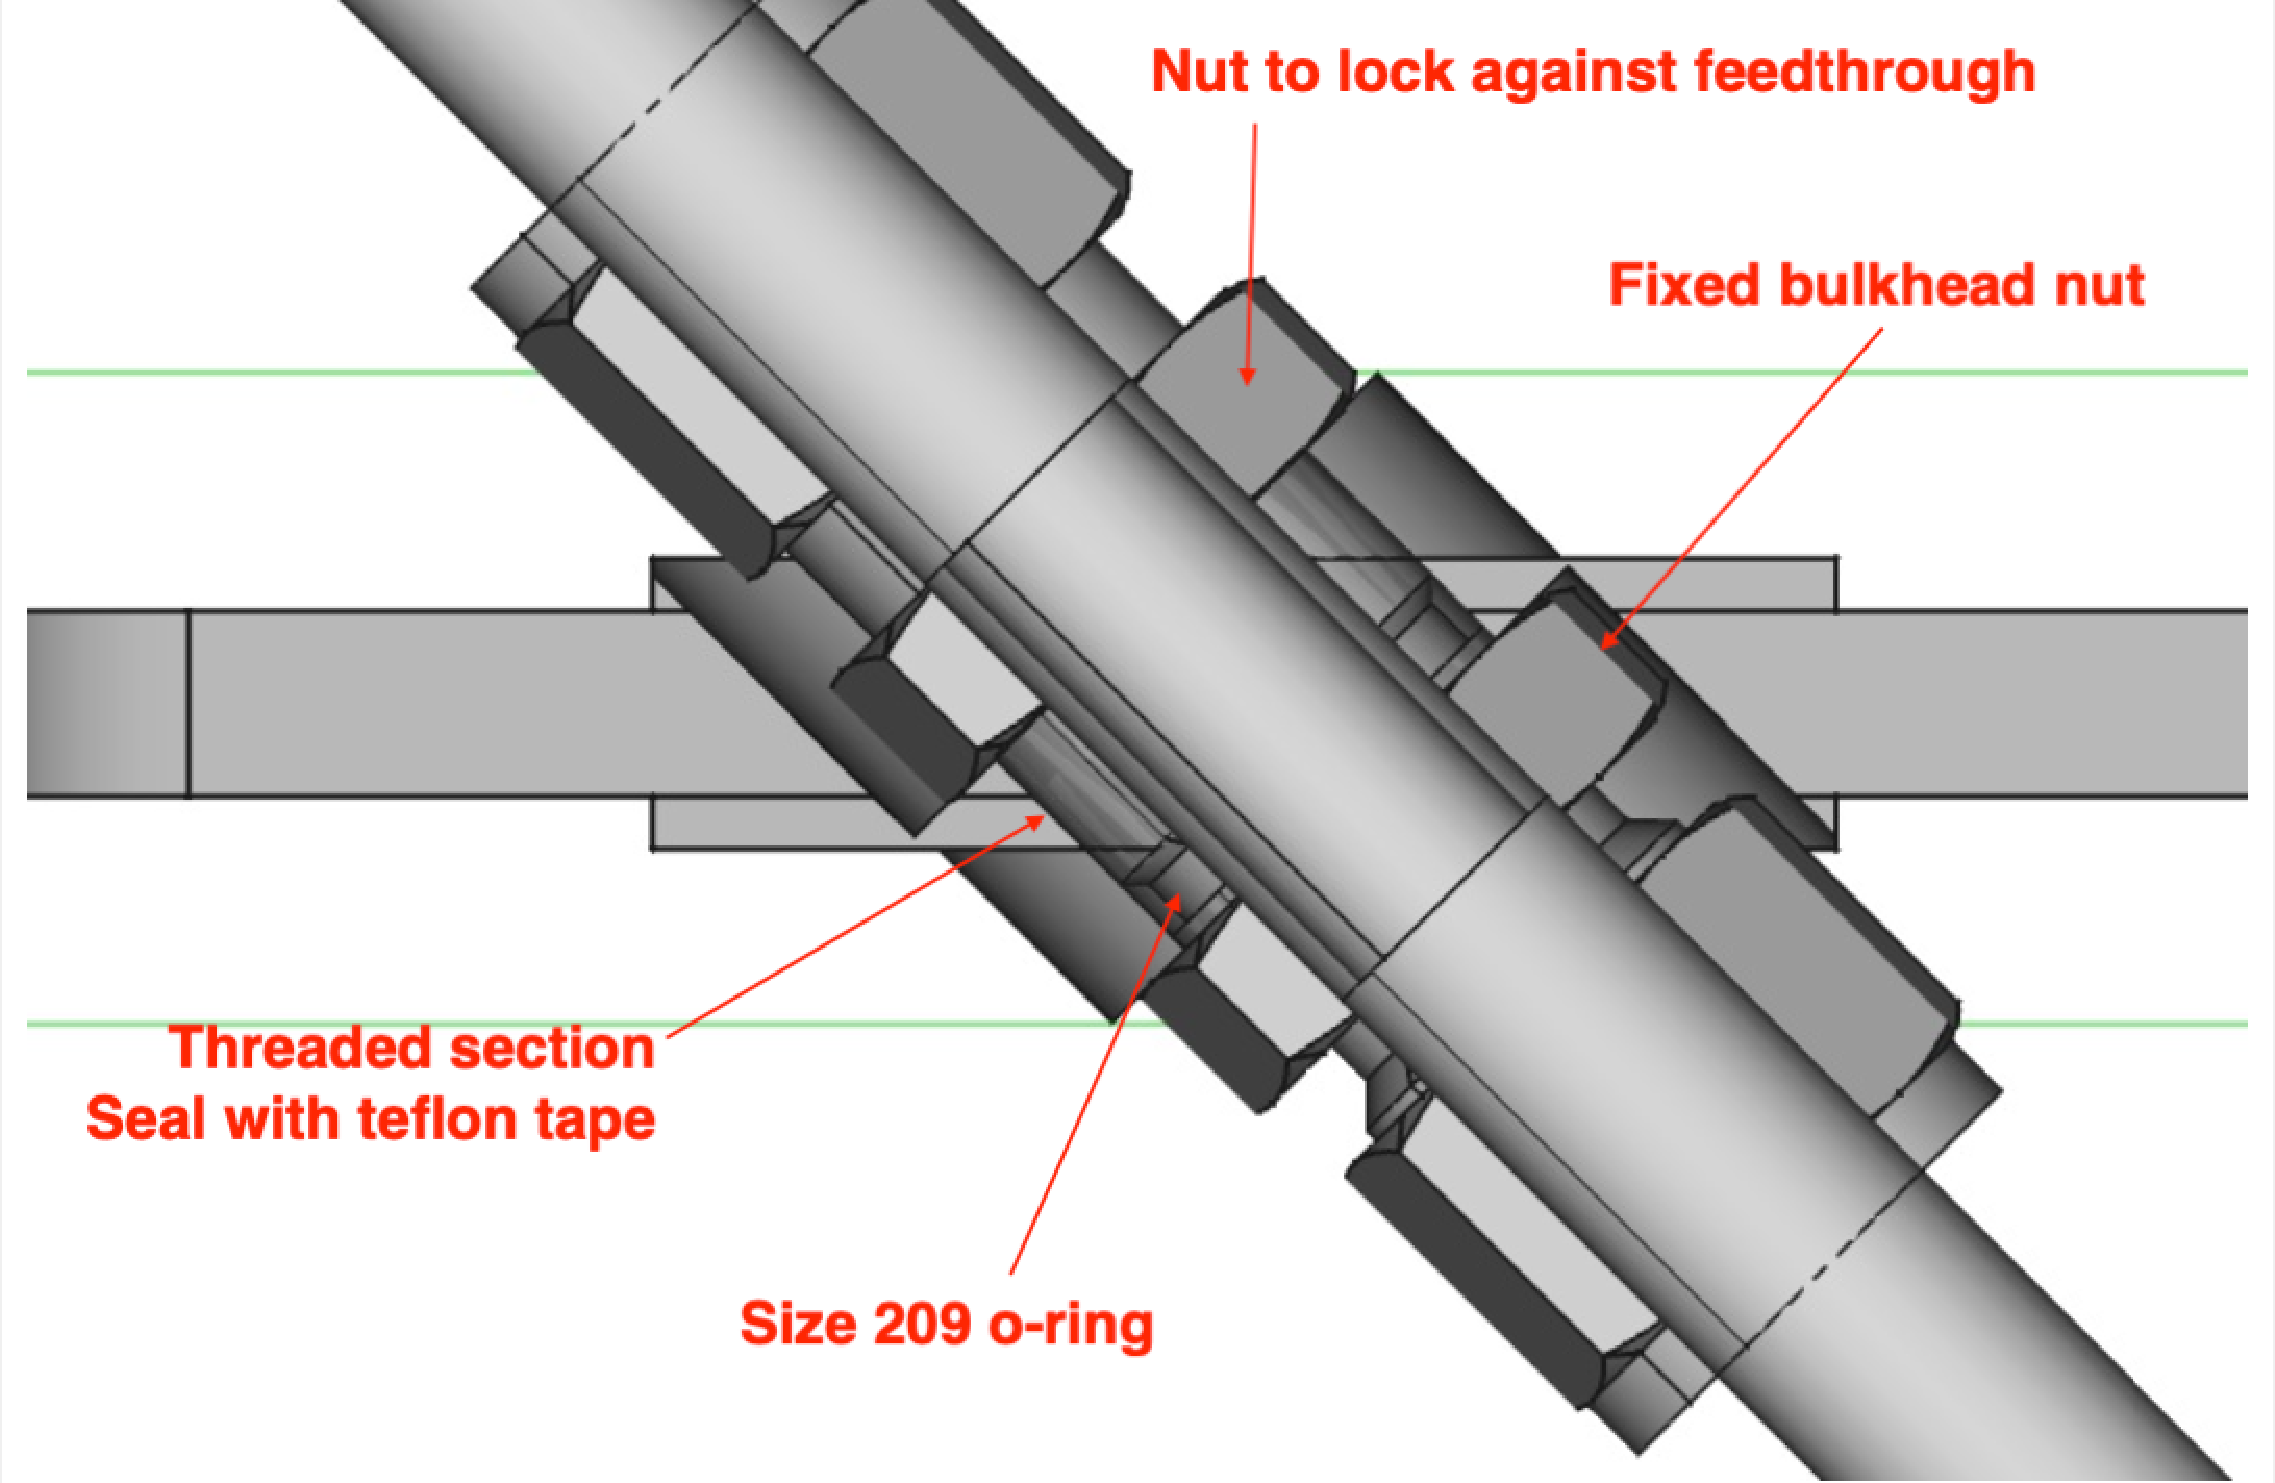
\includegraphics[width=\textwidth]{UmbilicalFeedthroughCutaway_2a.pdf}
      \caption{Cutaway view through the bulkhead and umbilical}
      \label{fig:UFCut}
    \end{subfigure}
  \end{center}
  \caption{A representation of the feedthrough plate. Measurements are estimated, but the dimensions of the bulkhead fitting are correct. This shows the degree of milling required to incorporate the bulkhead fitting.}
  \label{fig:UmbilicalFeedthrough}
\end{figure}

Tests have shown that the bulkhead fitting, when secured to the
umbilical using the two nuts and ferrules, does not move along the
umbilical when the umbilical was put under tension. 

To conduct this procedure the following items are required
\begin{itemize}[label=$\square$]
\item Cleaned, installed umbilical
\item 1/2'' through-bore bulkhead fitting (ultra-sonically cleaned)
\item Two 3/4'' ID FFKM o-rings
\item Two 1/2'' Swagelok nuts (ultra-sonically cleaned)
\item Two 1/2'' Swagelok teflon ferrules
\item Spray bottle of fresh UPW
\item Supply of Fisherbrand, Poly-celulose cleanroom wipes
\end{itemize}

To install the umbilical in this way, a worker must
\begin{answerlist}
\item Put on a double layer of clean-room gloves using the procedure in section \ref{ss:Rgloves}.
\item Wipe down the end of the umbilical that is to be secured to the
  feed-though with cleanroom wipes and UPW. 
\item Identify the location of the feed-through on the umbilical. This
  should be 3 meters from the end of the umbilical to provide space to
  produce the fibre bundle on the standing end of the umbilical and
  the same on the running end of the umbilical while allowing enough
  length to reach the bottom of the AV.
\item String a Swagelok nut, and ferrule onto the umbilical oriented
  to secure in the direction of the standing end.
\item Add an o-ring onto the bulkhead fitting and push it tight
  against the fixed nut. Thread the bulkhead fitting into the
  feed-through plate with the fixed nut side on the outside of the
  plate. Get the fixed nut as close to the exterior face of the
  feed-through as possible so that the o-ring is compressed.
\item Add an o-ring to the opposite side of the bulkhead fitting and
  press it against the inside of the plate. Tighten the opposing nut
  against the o-ring enough so that it is compressed; more is
  unnecessary and potentially difficult.
\item Run the umbilical through the combined bulkhead fitting and
  feed-through plate. String an additional Swagelok PTFE ferrule and
  stainless steel nut after the feed-through oriented so that the nut
  can tighten against the bulkhead fitting.
\item Place the feed-through on the umbilical at 3 meters from the end
  of the umbilical. This should be determined carefully with enough
  excess to run the umbilical properly with the URM as it will not be
  possible to reposition the umbilical after the following step. Note:
  there is a difference of 6 meters between the capacity of the URM
  and the total length of umbilical required to reach the bottom of
  the AV so additional length can be taken if necessary.
\item Move the inside ferrule up to the bulkhead fitting. Tighten the
  inside Swagelok nut onto the ferrule at the bulkhead fitting.
\item Move the outside ferrule up to the bulkhead fitting. Check that
  the umbilical is not experiencing tension or compression when the
  ferrule is tight against the end of the bulkhead. Tighten the
  outside Swaglok nut onto the ferrule.
\item With two M3 eye-bolts (already in place) and a piece of wire,
  suspend the feed-through on the URM from the hanger bar for the
  duration of the umbilical loading procedure. The feed-through should
  be placed so it can be reached when the cover is being replaced.
\end{answerlist}


\subsection{Rope Installation}\label{ss:RopeInstall}
The rope should be taken from the supply of Tensylon polymer rope kept
in the DCR. This rope has been stored on a spool that is maintained in
plastic bag inside the DCR. To spool the rope onto the URM the
following steps should be followed
\begin{answerlist}
\item Workers must don cleanroom gloves before handling the rope. A
  first pair must be rinsed with UPW before donning a second pair
  which must also be rinsed.
\item Collect roughly 40 m of Tensylon rope from the spool in the
  DCR. Fold the rope into a plastic bag to avoid knotting.
\item Clean the rope in an ultra sonic cleaner with a set of stainless
  steel weights and hooks. Cleaning will include one cycle with a
  mixture of nuclean and UPW and two rinse cycles using just UPW.
\item Once the ultra sonic cleaning is complete, the rope should be
  folded loosely in a plastic bag and dried out using a flow of
  nitrogen.
\item Tie a 30 cm segment of the cleaned rope from the eye-bolt
  supporting the sprung pulley to the pulley itself through the center
  of the spring. This will limit maximum extent of the spring.
\item Thread the rest of the cleaned rope through the hole at the top
  of the URM rope drum and secure the rope around the axis of the drum
  using a folded bow-line (see Fig. \ref{fig:bowline} for
  instructions).
\item Hold the rope perpendicular to the surface of the drum, start
  the rope motor running at 50 rpm. Verify that the drum is rotating
  in the appropriate direction so that the rope loads onto the drum
  consistent with the right handed screw grooves on the rope
  drum. Once the direction is verified to be correct, increase the
  motor rate to between 500 and 1000 rpm.
\item When the rope nears the end of the drum, slow down the motor and
  stop it when the rope is loaded down to the last groove.
\item With one person holding the rope tight to the spool so that it
  does not fall off, a second person must then string the rope through
  the pulley system. The running end of the rope should go over the
  pulley supported by the lead screw down to the rear fixed pulley
  near the URM bed, over the sprung pulley, back down to the front
  fixed pulley and up over the load cell pulley. before going down the
  URM access port parallel to the umbilical.
\item The slack through the rope system must be removed by tying
  cleaned rope hook to the rope and hanging a cleaned weight from the
  hook to maintain tension on the system until the source connector is
  secured to the rope.
\end{answerlist}

\begin{figure}
  \begin{center}
\begin{subfigure}{0.4\textwidth}
  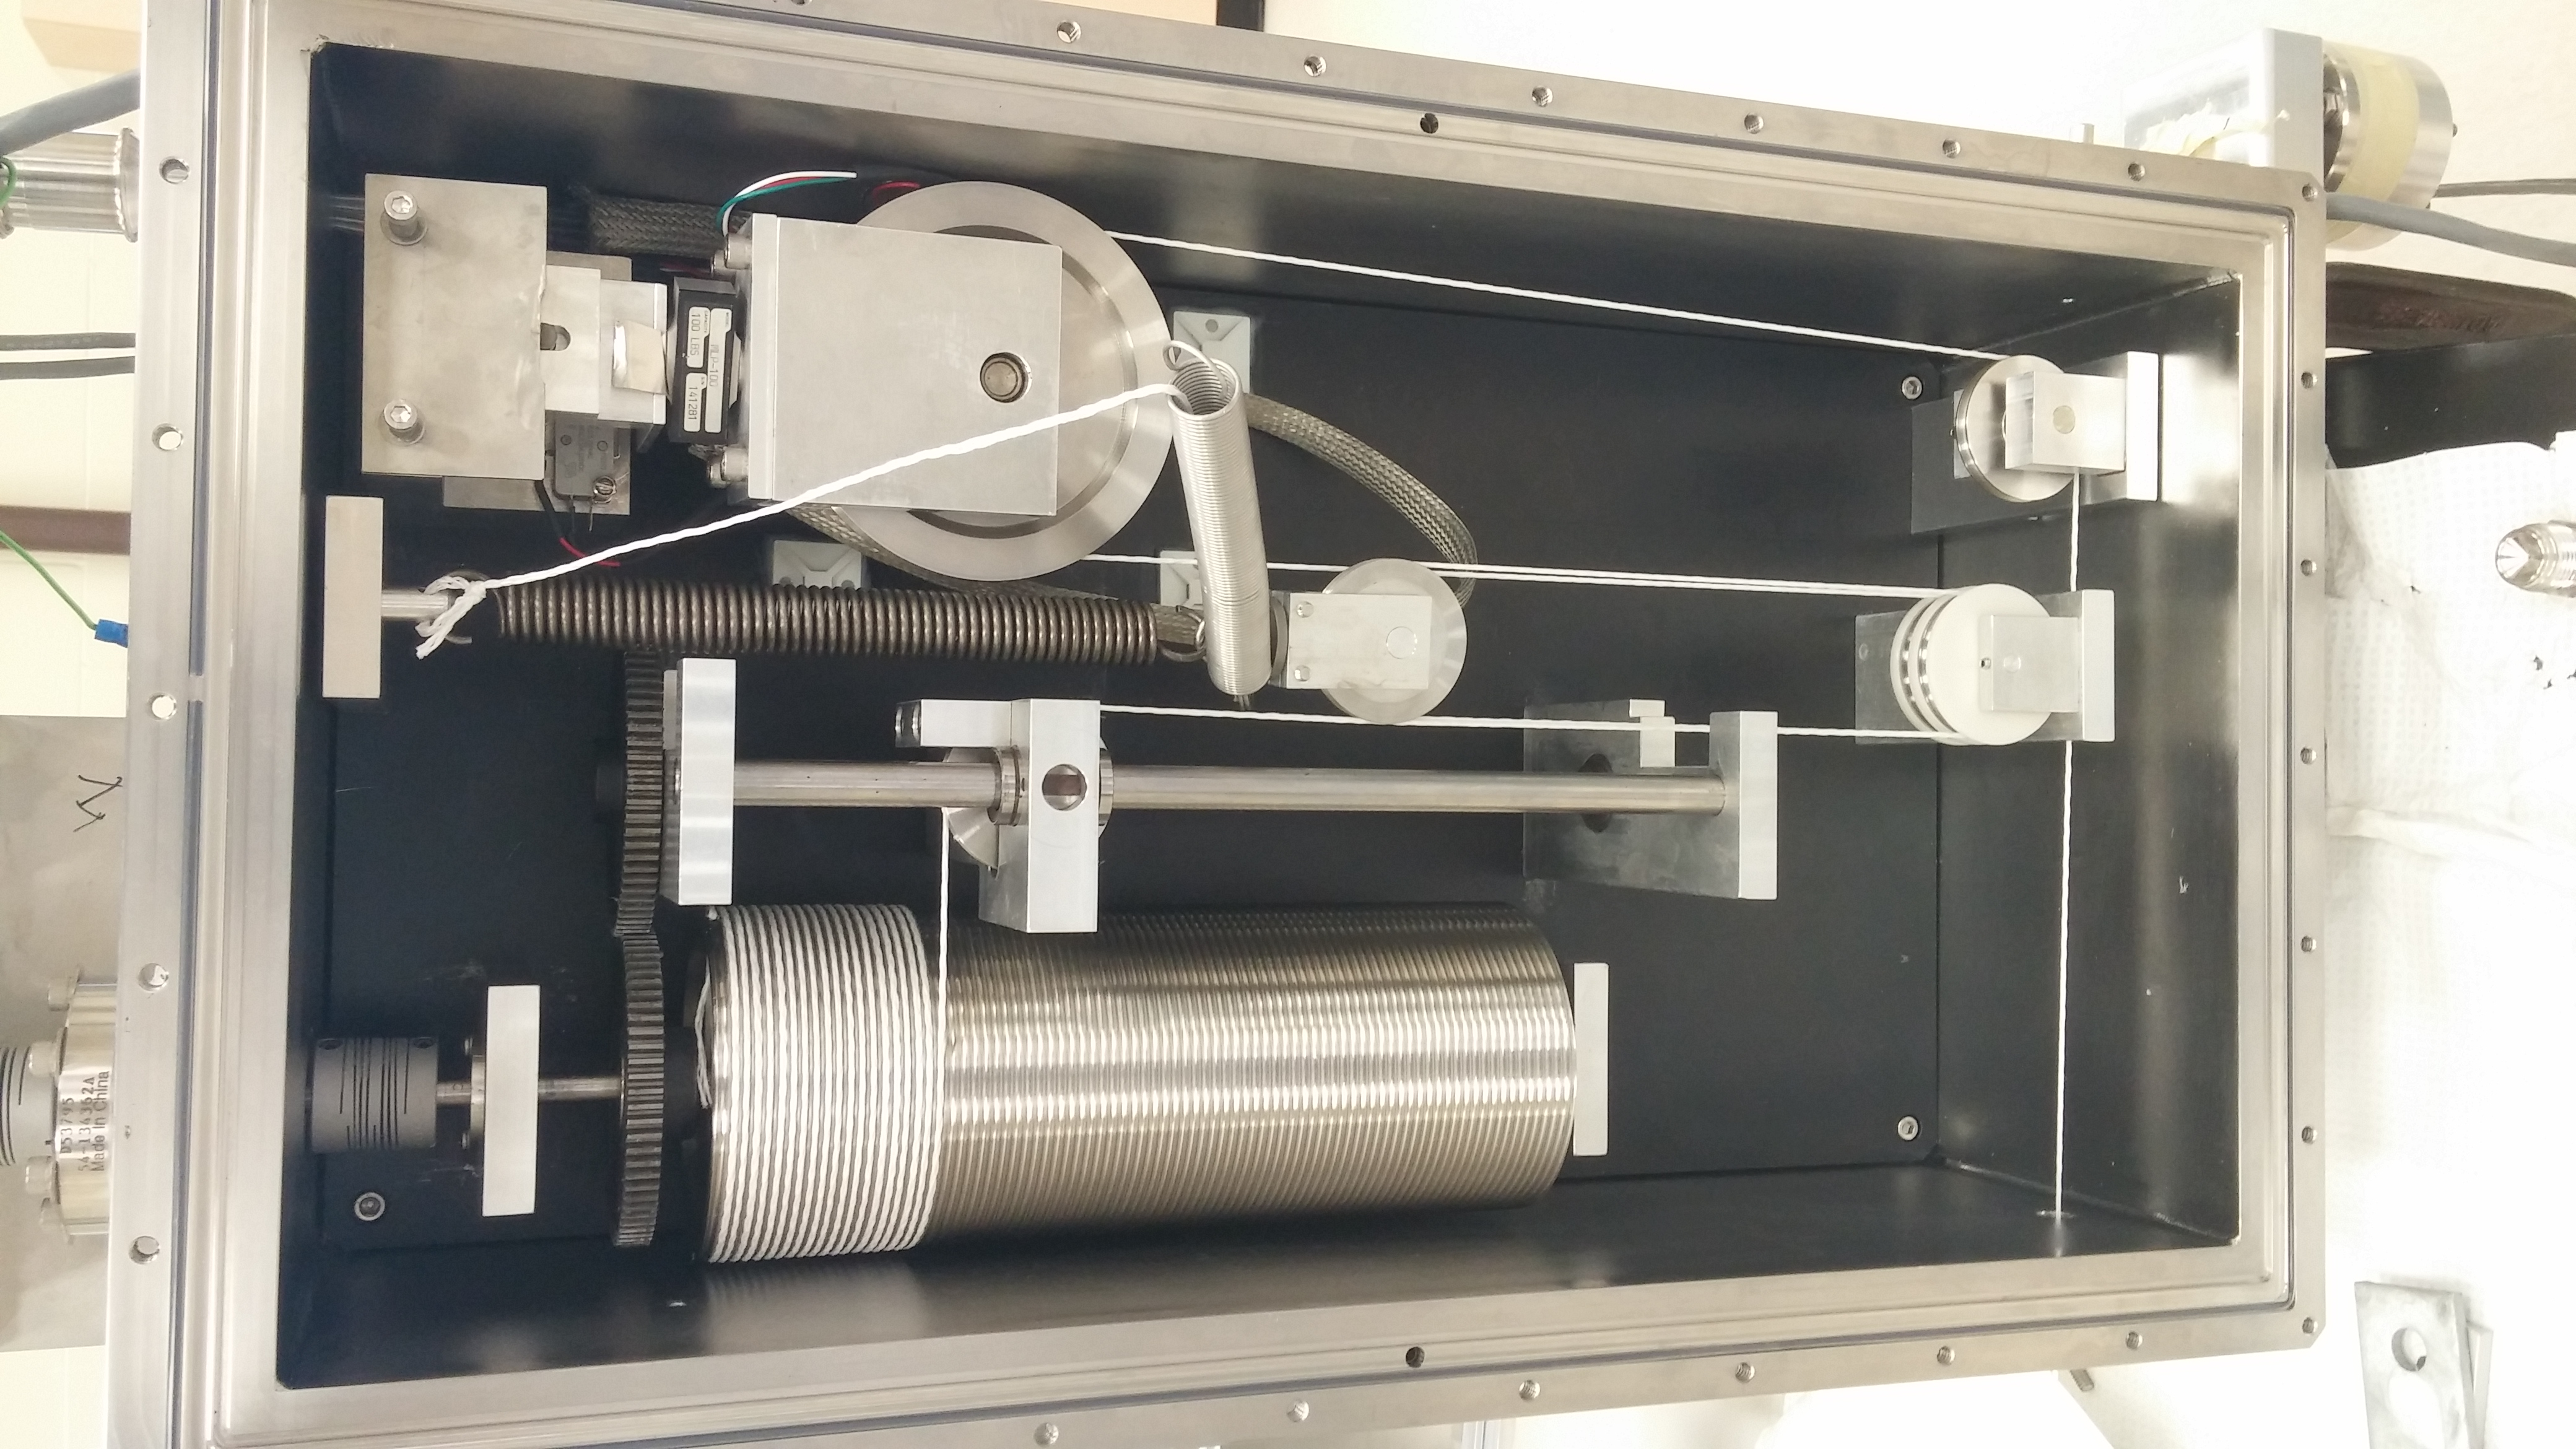
\includegraphics[height=\textwidth,angle=270]{RopeSystemMB}
  \caption{Rope system for a side rope motor box using a URM spring to support the sprung pulley. The URM rope system is identical except that the umbilical exit port on the URM is in the location of the final pulley on the rope box.}
  \label{fig:ropeSystem}
\end{subfigure}
\begin{subfigure}{0.5\textwidth}
  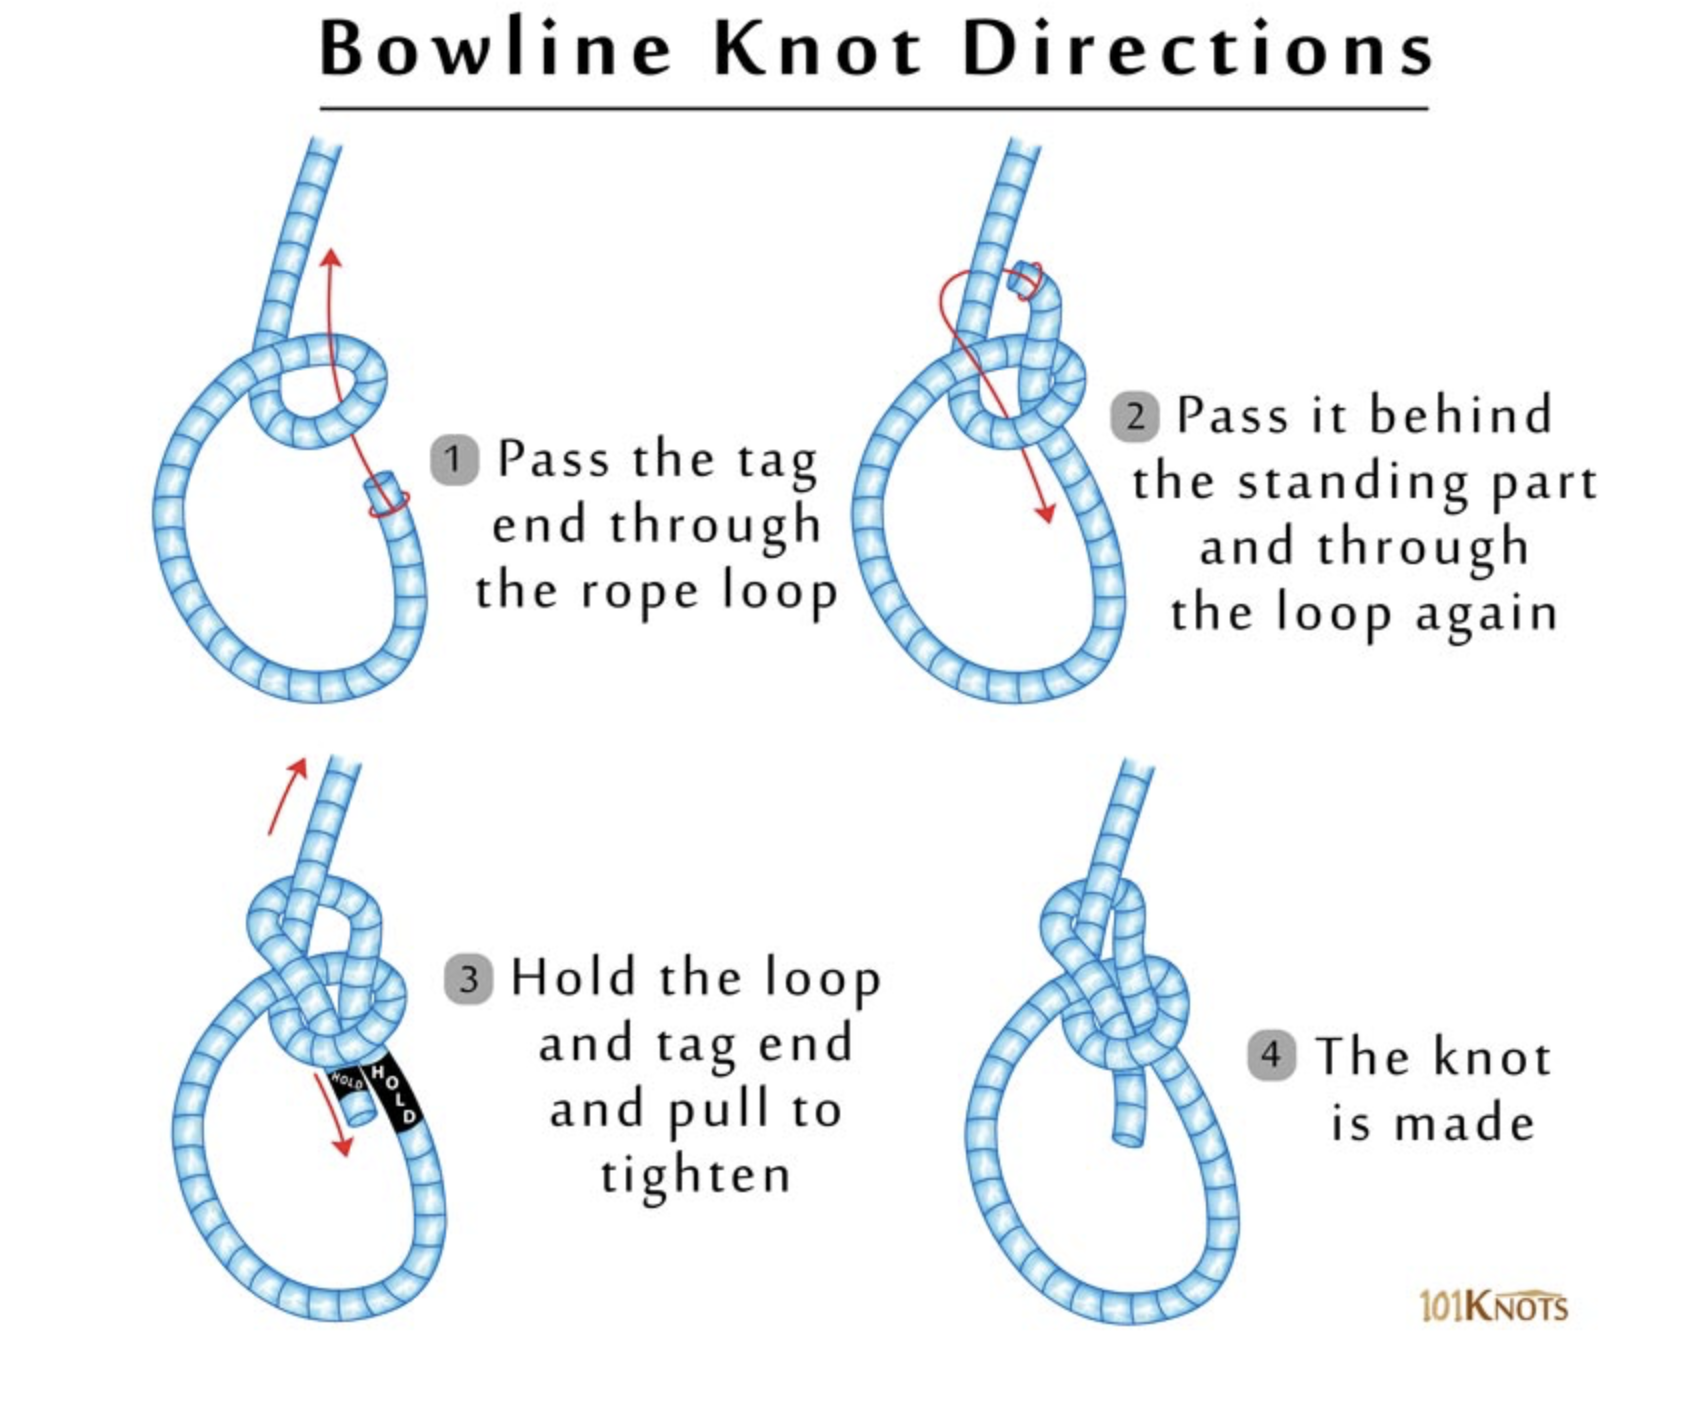
\includegraphics[width=\textwidth]{BowlineKnotDirections}
  \caption{Instructions for the knot to be used to secure the URM rope. Note a slightly easier method in this context is to tuck the standing end back through the loop at step one to make a bight. Then the running end is passed through the bight and the loop can then be placed in the desired location before the standing end is pulled tight to recreate the loop in step 3, above.}
  \label{fig:bowline}
\end{subfigure}
  \end{center}
  \caption{Details for the rope installation}
  \label{fig:rope}
\end{figure}



\subsection{Cover Installation}\label{ss:CoverInstall}
The following procedures to be completed with the URM in the following state
\begin{itemize}[label=$\square$]
\item The URM on the URM cart.
\item The URM cleaning is complete.
\item The umbilical and rope are installed on the URM.
\item The electrical and gas distribution systems have been checked and are in working order. 
\end{itemize}
\subsubsection{Mount the cover to the URM base}
\begin{answerlist}
\item Wipe the inside of the URM cover with UPW and clean room wipes.
\item Remove the bumpers from the edge of the URM flange.
\item Inspect the flange surface for imperfections and remove any
  traces of residue that may have been left on the surface by wiping
  with UPW or LAB.
\item Check that the o-ring remains properly installed and free of
  nicks or cuts.
  % \item Coil the length of umbilical above the feed-through plate and secure it temporarily inside the URM from the plate supporting the electrical and umbilical feed-through.
\item Insert the standing end of the umbilical (the one on the outside of the feed-through plate) into the appropriate opening in the URM cover from beneath (it is likely that this will be easier if the URM is on its side after cleaning. 
\item With four people (one on each corner) lift the cover over the
  back plane of of the URM.
\item A fifth person should watch the feed through plates to make sure
  they do not get caught on the cover as it descends. A sixth person
  should pull the umbilical out of the URM cover as it is lowered so
  that the fibre is not in risk of kinking. The remaining workers may
  then carefully lower the URM cover by the flange to provide an
  appropriate angle. It must be stressed that the motor box cover must
  go down straight over the back plane or it will get hung up.
\item The grips of the four workers lowering the cover should shift to
  use the lifting eye-bolts for the last few centimeters to avoid
  potential pinch points. The fifth worker should double check the
  status of the o-rings on the base flange before the cover is fully
  lowered.
\item Bolt the cover flange to the URM base. Each bolt must have a
  washer on the top and bottom and fastened with a nut. Initially only
  tighten the nuts to finger tight. There may be some movement in the
  flange so the best practice is to start from the middle of the URM
  on both sides and systematically work towards both ends in a
  staggered pattern.
\item With a crescent wrench and M5 hex wrench, tighten the bolts, again starting from the middle and working towards the ends. A third pass (without over-tightening) is encouraged.
\item Connect the vacuum leak checker to one of the flange VCR ports
  connecting to the inter o-ring space. Systematically test the flange
  with a helium probe. A leak rate greater than 10$^{-7}$ mbar L/s
  should be treated as a fail. The likely fail case is due to a
  displaced o-ring; the flange should be disassembled, the o-rings
  should be inspected and if the o-rings are still considered ``good''
  the flange can be re-assembled. If there are any cuts or
  deformations in either o-ring, the o-ring must be replaced, using
  the o-ring from URM5. Then the flange can be reassembled as before.
\end{answerlist}
\subsubsection{Install the electrical feed-through}
\begin{answerlist}
\item Pull the o-rings for the electrical feed-through flange out of
  their storage bag. Check the o-rings for nicks and cuts. If there
  are any the o-ring must be replaced.
\item Wet the o-rings with LAB and place them in the electrical
  feed-through groove. This is done so that they will stick in the
  o-ring grooves when the plate is held vertically. The operator
  should hold the plate by the feed-through and inter o-ring VCR ports
  against the inside of the cover once the o-rings are placed to
  ensure that they do not have a chance to leave the groove. Every
  effort should be made to avoid letting the o-ring drop into the URM
  cover as it will be extremely difficult to retrieve it. The best way
  to achieve this is to always keep a grip on the electrical feed-though
  and maintain pressure against the cover.
\item A second operator should sightly grease the threads (only) of
  the 26 M4 screws with Super Lube. That operator must change outer
  gloves after the screws are greased to reduce cross contamination.
\item The second operator will bolt the feed-through plate to the
  outer cover. Because the flange is bolted to the inside of the cover
  using blind holes, it is important to make sure that all of holes
  are correctly aligned before tightening the flange. While the first
  operator holds the flange against the inside of the cover to reduce
  the chance of the o-ring falling out, the second operator must start
  all of the screws in their blind holes, but not tighten them.
\item With the first operator still maintaining pressure between the
  plate and the cover, the second operator must tighten all the screws
  to finger tight in a star pattern to maintain even pressure on the
  flange. 
\item With the appropriate hex wrench, tighten all of the bolts with
  by no more than 2 turns in a star pattern. Once complete, continue
  the star pattern by an additional half turn or more to tighten the
  screws without over tightening. The first operator can now release
  the plate.
\item Connect the helium vacuum leak checker to one of the VCR ports
  on the flange connecting to the inter o-ring space. Systematically
  test the flange with a helium probe. A leak rate greater than
  10$^{-7}$ mbar L/s should be treated as a fail. The likely fail case
  is due to a displaced o-ring; the flange should be disassembled, the
  o-rings should be inspected and if the o-rings are still considered
  ``good'' the flange can be re-assembled. If there are any cuts or
  deformations in either o-ring, the o-ring must be replaced. Then the
  flange can be reassembled as before.
\end{answerlist}
\subsubsection{Install the umbilical feed-through}
\begin{answerlist}
\item One operator must lightly grease the 14 M4 cap screws required for the
  installation of the umbilical feed-through plate with Super
  Lube. Change outer gloves.
\item A second operator must extract the o-rings for the umbilical
  feed-through plate from its storage bag and lubricate the o-rings
  with LAB. Hold the o-rings so they do not touch any other surfaces. 
\item The first operator must pull the umbilical through the o-rings
  while the second operator carries the o-rings towards (but not
  touching) the URM cover. 
\item The first operator must carefully extract the umbilical
  feed-through from inside the cover. The second operator must install
  the o-rings while the feed-through is held by the VCR ports by the
  first operator. The second operator should change outer gloves after
  the o-rings are in place
\item The first operator must pull the umbilical feed-through plate
  against the inside of the cover to keep the o-rings in place.
\item The second operator must
  start all of the screws in the threaded holes in the plate.
\item While the first operator maintains pressure between the plate
  and the cover, the second will systematically tighten the screws to
  finger tight.
\item Working in a star pattern with a hex wrench, tighten the screws
  by an equal amount (no more than two turns). Continue the star
  pattern to ensure that all of the screws are tight without
  over-tightening. The first operator can now release pressure on the
  plate.
\item Connect the vacuum leak checker to one of the VCR ports on the
  umbilical feed-through flange connecting to the inter o-ring
  space. Systematically test the flange with a helium probe. A leak
  rate greater than 10$^{-7}$ mbar L/s should be treated as a
  fail. The likely fail case is due to a displaced o-ring; the flange
  should be disassembled, the o-rings should be inspected and if the
  o-rings are still considered ``good'' the flange can be
  re-assembled. If there are any cuts or deformations in either
  o-ring, the o-ring must be replaced. Then the flange can be
  reassembled as before.
\end{answerlist}

\subsection{Transfer the URM to the Lifting Table}\label{ss:transfer}
The URM currently sits on one of the SNO carts in the DCR. This allows the URM to be worked on at a more reasonable height than the resting height of the lifting table. However, once the cover is on the URM should be transferred to the lifting table for all further steps. This is a six person task led by a calibration expert.  
\begin{answerlist}
\item Wrap the gas outlets on the bottom of the URM with plastic
  encapsulated foam to cushion any contacts with the gas manifold
  through the following procedure.
\item Two workers orient the URM cart with respect to the lifting
  table so that front of the URM is facing the back (handle side) of
  the lifting table.
\item Lift the URM until it is at the same height as the lowest height
  of the lifting table.
\item Engage the breaks on the lifting table and the URM cart. Two
  workers must brace the lifting table so that it does not move
  through the next steps.
\item Detach the chains securing the URM to the cart.
\item Push the URM from the cart to the lifting table. Two workers
  should hold the URM cart and push the URM forward while two more
  workers guide the URM onto the lifting table.
\item The workers holding the cart must be sure to stop the forward
  motion of the URM before the gas connections reach the URM cart. The
  URM center of mass should be over the lifting table at this point.
\item The rear workers must hold the URM back end up while the two
  workers steadying the lifting cart remain in place. The two
  remaining workers should lower the URM cart and remove it from the
  working area.
\item The rear workers and the free workers must finish moving the URM
  onto the lifting cart, while the workers holding the lifting table
  stay in place. The final location for the center of mass is shown in
  Fig. \ref{fig:URMpreBellows}.
\item Once the URM is in position secure the URM to the lifting table
  using the appropriate chains and turnbuckles.
\item Connect the wheel mounts to the URM in the appropriate positions using the URM flange bolts to secure the outer sides of the plates. Install the inner, plates with the appropriate hex screws and connector bolts that pass through the URM skid wheel holes. Install the wheels with the bearings through the holes at the bottom of the mounts. 
\end{answerlist}


% \subsection{Source Tube / Bellows Installation}

\subsection{Source Tee Installation}\label{ss:SourceTeeInstall}
%This procedure assumes that the bellows cleaning and leak checking is complete.
The bellows and associated hardware arrived in the SNOLAB underground lab in March of 2022. They were cleaned in the control room, double bagged (using large clear plastic bags) and stored in the DCR over the course of two nights.

The source tee installation must be conducted before the source
connector is installed. The umbilical path hole, while wide relative
to that for the water URMs is not wide enough for the pulley assembly
of the source connector. The source tee cannot be installed until the
URM has been moved to the URM lifting table.

Required for this procedure are
\begin{itemize}[label={$\square$}]
\item URM with the cover on
\item The source tee flange
\item Source tee flange bolts (already on the URM)
\item 13mm Hex Wrench
\item teflon encapsulated viton and viton o-rings
\end{itemize}

\begin{answerlist}
\item Unwrap source tee flange.
\item Wipe all surfaces of the flange with UPW.
\item Place o-rings on the top of the source tee using a little vacuum grease on the viton o-ring and LAB on the teflon encapsulated o-ring to ensure they remain in place.
\item Carefully place the lower end of the umbilical and the weighted rope through the center of the tee-flange. Avoid getting any of the lubricant on either the rope or the umbilical.
\item Remove the source tee flange bolts from the bottom of the URM.
\item With one person to hold the source tee, raise the source tee up
  to the bottom of the URM. Orient the tee 60 degrees from the
  backwards direction of the URM to the right, so that the view port
  will face in the SSW direction when the URM is mounted. Start all
  bolts on their threads
\item Tighten the bolts in a star sequence so the source tee compresses its o-rings against the bottom of the URM.
\item Install the source tee window on the view port of the source tee flange.
\item Connect the vacuum leak checker to one of the source tee inter
  o-ring test ports. Systematically test the edge of the flange
  against the URM with the helium probe. The leak rate must be less
  that 10$^{-7}$ mbar L/s. If the test fails the source tee flange
  must be disconnected and the source of the leak must be identified
  before re-installing the source tee flange.
\end{answerlist}

\subsection{Source Connector Installation}\label{ss:SourceConn}
Assembly of the source carriage requires the cleaned and installed
umbilical and central rope. The source connector was machined and
electro polished at U of A before it was sent to Sussex for the UFO
construction and testing. It was then sent to Queen's with the
Laserball source before coming to Sudbury when the Laserball fill
tests began. It was cleaned with all of the Laserball parts prior to
the initial fill.

A limited assembly test showed that the source carriage design that
included the UFO would not work because the acrylic piece had warped,
so that the diameter of the lip on both sides would not admit the top
and bottom plates. For this reason, a new top plate has been designed
that provides a platform to clamp onto the umbilical which can be
bolted to the source connector and the rope pivot. The following
installation procedure assumes the installation of the new plate.

The procedure also assumes that the fibre bundle has been consolidated
in an epoxy filled pipe, the procedure of which will be described
elsewhere and should be done by specific laserball experts. The
procedure of producing that fibre bundle involves sanding the end so
steps must be taken to protect the URM interior during that process
and clean the umbilical after. The procedure can in principle be
completed without the fibre bundle in place in preparation for AmBe
source deployment, but the end of the umbilical must be left free.

\begin{answerlist}
\item Wet the bottom meter of umbilical with LAB
\item Pre-wet all of the screws with LAB
\item Install o-rings on the upper source connector body 
\item Thread the umbilical through the pivot
\item Thread the umbilical through the three pressure plates with a teflon o-ring following each one.
\item Thread the umbilical through the top plate of the source connector.
\item Ensuring that there is a surplus of umbilical below the top
  plate of the UFO run the umbilical through the UFO acrylic, steel plate and stainless steel cylinder. $\sim$5cm of Tygothane cladding below the top plate followed by 10 to 30 cm of exposed fibre.
\item Feed the spring cap followed by the fibre spring through the exposed fibres.
\item Prepare the station for completing the fibre bundle. Have the fibre cable shroud, epoxy, and a 1 mL plastic syringe ready.
\item Mix the epoxy as directed and draw $\sim$1 mL into the plastic syringe. Slide the fibre cable shroud onto the fibres as you inject the epoxy continually until the bundle is filled.
\item Ensure all fibres reach the end of the fibre bundle. Leave the fibre bundle for curing. \textit{Note: this may take several days but can be expedited by setting up a heat gun to provide a warmer environment.}
\item Once cured, set up the station for cutting the fibre bundle. This involves a dremel with a diamond dremel bit, plastic bundle rig, and vacuum. Secure the dremel with a c-clamp and install the diamond bit.
\item Place the fibre bundle in the plastic bundle rig. The purpose of this is to distance the operator from the dremel bit and ensure a perpendicular cut. One operator guides the plastic rig along the dremel bit while the other operator deploys the vacuum.
\item Prepare the polishing station. It is helpful to have a retort stand and clamp hold the umbilical upright with the fibre bundle directed downwards. This allows for the sandpaper to be placed underneath and the fibre bundle goes into the sanding puck while minimizing the load on the bundle.
\item Using UPW to wet the carbide sandpaper progress from 400 to 4000 grit sandpaper in progressive increments. At 4000 grit, use the 1 micron polishing compound. After polishing a quick test with a cap lamp at one end can verify quality.
\item The fibre bundle is now complete. Bring the spring and spring cap to the fibre bundle.
\item Secure the fibre connector top plate to the source upper source
  connector body with 8 M3 screws.
\item Couple the end of the fibre via two M3 screws on spring cap onto the fibre connector top plate. Connect the wires to the further electical feedthroughs on the source connector plate.
\item Fasten the upper source connector plate to the top of the upper source connector body using 8 M3 screws. These screws must include holes for retaining wire. The retaining wire should be installed at this time.
\item Tighten the pressure plates against the top of the source
  connector top plate.  using six \#4-40 1 inch length screws until
  there is an equal gap less than 1 mm between all of the plates. The
  mounting screws must have a hole for a retaining wire, and that wire
  should be installed after
\item Secure the source pivot pulley support plates to the UFO assembly using four M3 screws. Retaining wire should be strung between the screws, which should also be equipped with holes to accommodate the wire. 
\item Tie the central rope to the rotating collar on the pivot
  assembly underneath the rope groove using a bowline tight against
  the barrel of the pivot. This should be done using the alternative
  method of tying the knot described above and should be tied so that the knot cannot go above the edge of the rope groove on the barrel.
\end{answerlist}

\begin{figure}
  \begin{subfigure}{0.5\textwidth}
  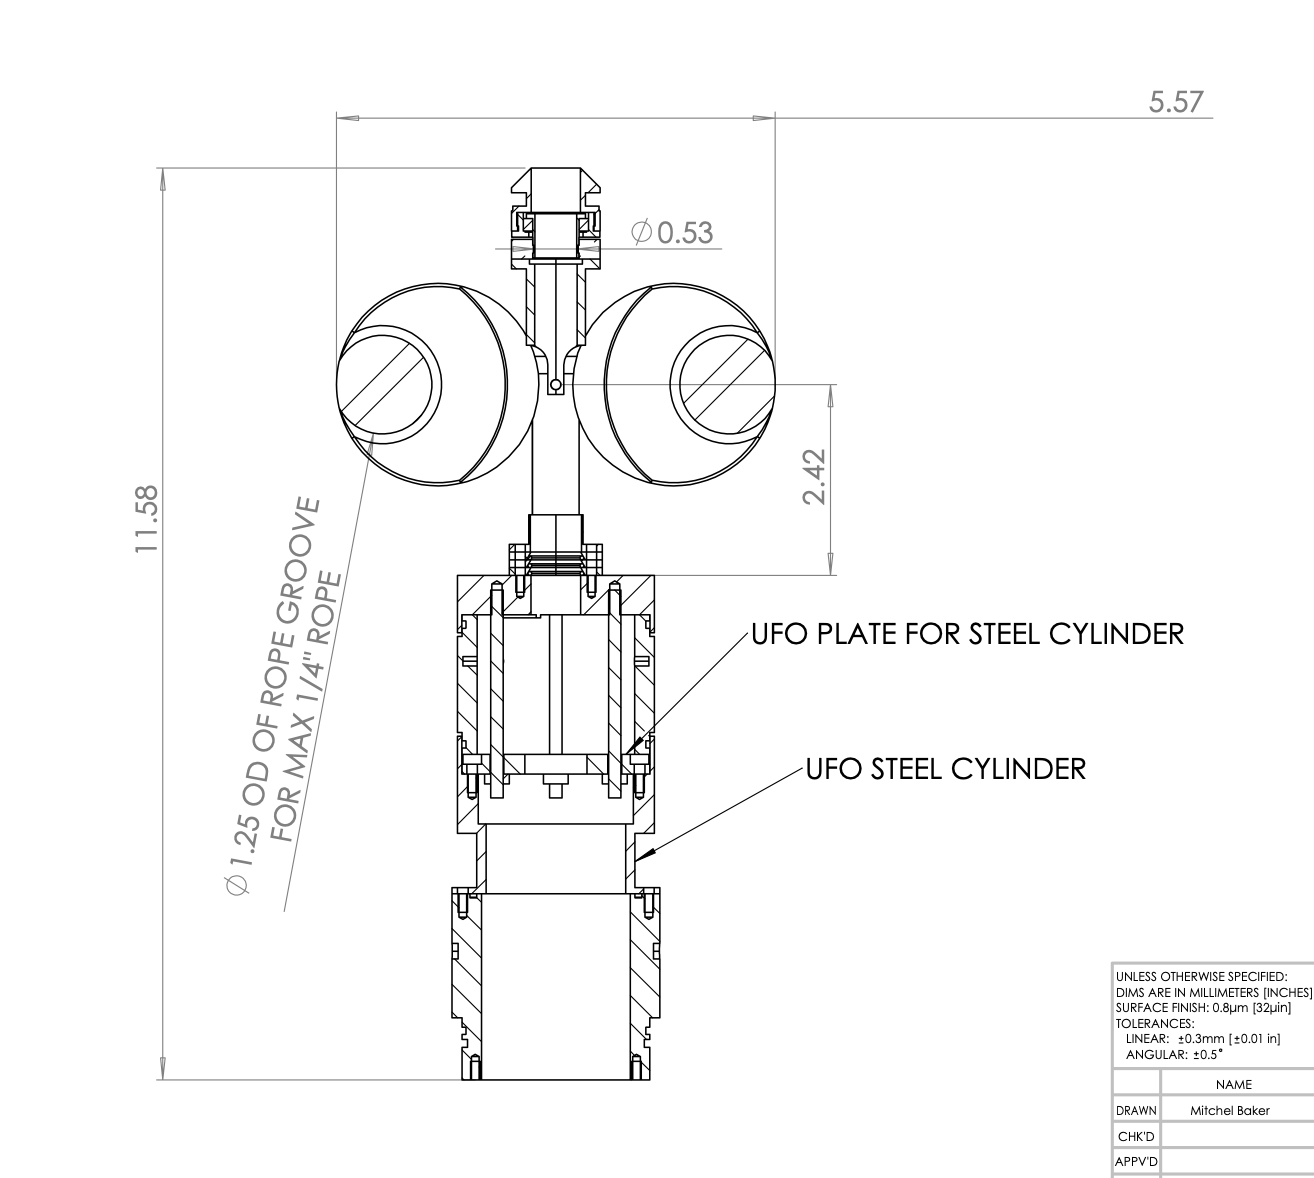
\includegraphics[width=\textwidth]{UFOPivotSourceConnector}
  \caption{The source pulley assembly with the UFO and top source connector.}
  \label{fig:Pivot}
\end{subfigure}
\begin{subfigure}{0.45\textwidth}
  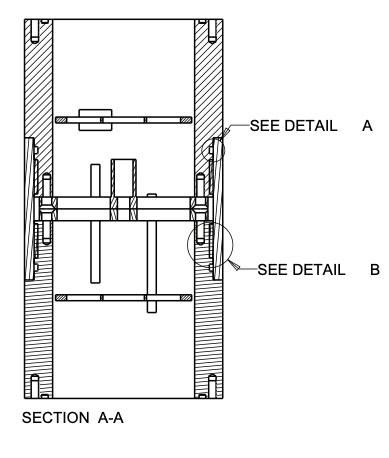
\includegraphics[width=\textwidth]{SourceConnectorSection}
  \caption{The source connector}
  \label{fig:sourceConn}
\end{subfigure}
\caption{The original plan to terminate the umbilical includes the source pulley assembly, a umbilical flasher object and a source connector as shown}
\end{figure}


\subsection{Final Umbilical Cleaning}\label{ss:UmbClean}
The Umbilical must be wiped with a LAB soaked lint free cloth during
loading. However, it cannot be assumed that all external material was
removed from the umbilical from this process. For this reason, soaking
the umbilical prior to deployment is considered the optimal method for
a final cleaning as it has the potential to remove remaining traces of
contamination from the umbilical in an environment comparable to the
AV. Assuming that the umbilical is installed on the URM with the
source connector blanked off (and the source tee is installed without
the bellows) the following procedure can be followed.
\begin{answerlist}
\item Clean the umbilical cleaning vessel (stainless steel stock pot) with soap (Sunlight) and water. Clean again with Nuclean and water in a 1:50 dilution. Rinse inside and outside with UPW twice. Wipe clean with UPW and lint free wipes. 
\item Fill the pot with 20-30 L of scintillator plant LAB. Retain a sample for liquid particle count for reference.
\item Position the pot under the URM umbilical exit port and lower the source connector into the pot.
\item Put the umbilical and rope into constant tension mode with a tension less than the weight of the source connector (20 N on each should be sufficient). Pull the umbilical down from the URM and coil the umbilical in the pot below the scintillator level.
\item Continue pulling the umbilical down until the manip system
  indicates that the moving block reaches the endpoint of the
  track. Stop all URM commands. {\bf The umbilical cannot be released until
    the URM stop command is issued.} Clear the error and return the
  rope to constant tension mode with a value less than the connector
  weight (20 N).
\item Using the Genie lift, raise the cleaning vessel up to the end of the source tee flange. Ensure that the umbilical settles into the pot while the rope retracts into the URM.
\item Close the gap between the URM source tee flange and the umbilical cleaning vessel so that all of the umbilical that can be deployed into the AV will be exposed to the LAB
\item Leave the umbilical in the LAB for 1 hour. 
% \item Leave the umbilical to soak for a week
\item When the umbilical cleaning is complete, ensure that the rope is in constant tension mode. Lower the umbilical cleaning vessel to the floor.
\item Submit a sample of the LAB for liquid particle counting. If the count does not conform to the particle standard relative to the reference sample, remove the LAB from the cleaning volume using a peristaltic pump and fill the cleaning volume with clean LAB and soak the umbilical for an additional hour. 
\item Connect the URM LAB drain ports to a vessel to collect the LAB as it drips off of the umbilical.
\item Put the umbilical into constant tension mode with a value greater than 20 N. The umbilical should retract into the URM at a reasonable rate.
\item Don PE gloves over the clean-room gloves. Watch the umbilical and try to remedy any tangles with a minimal amount of manipulation of the umbilical.
\item Allow the umbilical and rope to continue retracting into the URM stop the movement of the umbilical before the source connector assembly reaches the URM base plate.
\item Raise the umbilical cleaning vessel back up to the source tee flange to collect the LAB as it drips off of the umbilical and out of the URM.
\end{answerlist}
  

\subsubsection{Bellows installation}\label{sss:BellowsInstall}
Installation of the bellows should be paused to allow for the
installation of the source connector. This will allow for better
control of the umbilical and the rope during the bellows installation
and it is easier to conduct the source connector installation when the
end of the source tube is higher up. Similarly the umbilical soak
should be completed prior to the bellows installation.

The bellows was transported with three support struts welded onto the
support ring at the top and the bottom of the o-ring. These support
struts were painted yellow by the manufacturer. The paint can be
rubbed off with effort so there is concern that it could spread in the
DCR. For this reason the struts were wrapped with JamMek plastic to prevent
such contamination during storage. The struts will have to be removed
to allow the bellows to be used, but will be kept through installation
for stability.

For installation of the source bellows the following items are required
\begin{itemize}[label=$\square$]
\item Source bellows
\item Genie lift
\item 6 bolts and nuts required for the rotatable flange to bellows connection
\item teflon encapsulated viton and viton o-rings for bellows flange surface
\end{itemize}
\begin{answerlist}
\item Clean and install the Genie lift plate on the forks of the Genie lift if is not already there.
\item Place the Genie lift near the motor box end of the URM 90 degrees to its axis.
\item Cut and secure a piece of plastic onto the plate to prevent damage to the the bottom flange sealing surface.
\item Carefully position the bellows on the Genie lift and move the bellows underneath the source tee flange with the holes lined up between the bellows top flange and the rotatable flange. Always have one person holding the bellows so that it does not tip.
\item Place the o-rings in the groove on the top bellows flange.
\item  Slowly lift the bellows into position below the tee flange. When the two surfaces are 1~cm apart, insert the bolts through the flanges from the top down. Start threading the nuts and washers onto the bolts until the bolts are in contact with the lower surface of the flange.
\item Lift the bellows to allow for the bolts to be tightened by 2 to 3 thread widths. Continue until the bellows makes metal to metal contact with the source tee.
\item Tighten the bolts in a star pattern so that the bellows o-rings are compressed.
\item Install turn-buckles and cables between the bellows support
  rings. Tighten the turn-buckles until the wires are just tight
  between the support rings. These turnbuckles are intended to support
  the gate valve once it is installed.
 \item Connect the vacuum leak checker to one of the top flange inter
  o-ring VCR ports (with the other blanked off). Test the edge of the
  flange with the helium probe. The connection fails if the leak rate
  exceeds 10$^{-7}$ mbar L/s. If there is a failure the source must be
  identified and the bellows re-installed with a successful leak
  check.
\item Remove the support struts with bolt cutters or a hack saw
  breaking the top welds first and the bottom welds second. The strut
  must be held by a second person so that its movement is
  controlled. If a hack saw is used the bottom of the bellows must be
  blanked off to protect the interior of the URM and a vacuum cleaner
  must be run next to the hack saw blade to limit the spread of dust
  in the DCR.
\item Bag the struts and remove them from the DCR at the first opportunity.
\end{answerlist}
\subsection{Gatevalve Installation}\label{sss:GateValveInstall}
The gate valve arrived from the supplier in the fall of 2019. It was
subsequently sent underground in the shipping packaging in the summer
of 2021. Standard car wash procedures were followed when the gate
valve entered the lab including a full cleaning after removing the
packaging and swipe tests to confirm that surface contamination was
removed. Following that it has been stored in the DCR and wiped clean
several times.

This procedure can be done after the bellows is installed on
the URM. 
\begin{answerlist}
\item Clean and install the Genie lift plate on the forks of the Genie lift if is not already there.
\item Cut and secure a piece of plastic onto the plate to prevent damage to the the bottom flange sealing surface.
\item Maneuver the Genie lift to the shelf holding the 10 inch gate valve. Transfer the gate valve to the Genie lift.
\item Lower the gate valve as low as the Genie lift allows
\item Place the gate valve below the bellows.
\item Install the o-rings in the groove on the top side of the gate valve. 
\item Lift the gate valve to the bellows. Adjust the position of the
  bellows so that the holes on the gate valve matches those on the
  bellows. The body of the gate valve should be parallel to the URM,
  with the handle end directly below the stretcher box.
\item Bolt the bellows to the gate valve using the appropriate bolts with washers in place. Thread all of the bolts into the gatevalve to finger tight before systematically tightening all of the bolts in a star pattern.
 \item Connect the vacuum leak checker to one of the bottom flange inter o-ring VCR ports (with the other blanked off). Open the gate valve before starting the vacuum cycle on the leak checker. Test the edge of the flange with the helium probe. The connection fails if the leak rate exceeds 10$^{-7}$ mbar L/s. If there is a failure the source must be identified and the gate valve re-installed with a successful leak check. 
\end{answerlist}

\begin{figure}
  \begin{subfigure}{0.9\textwidth}
    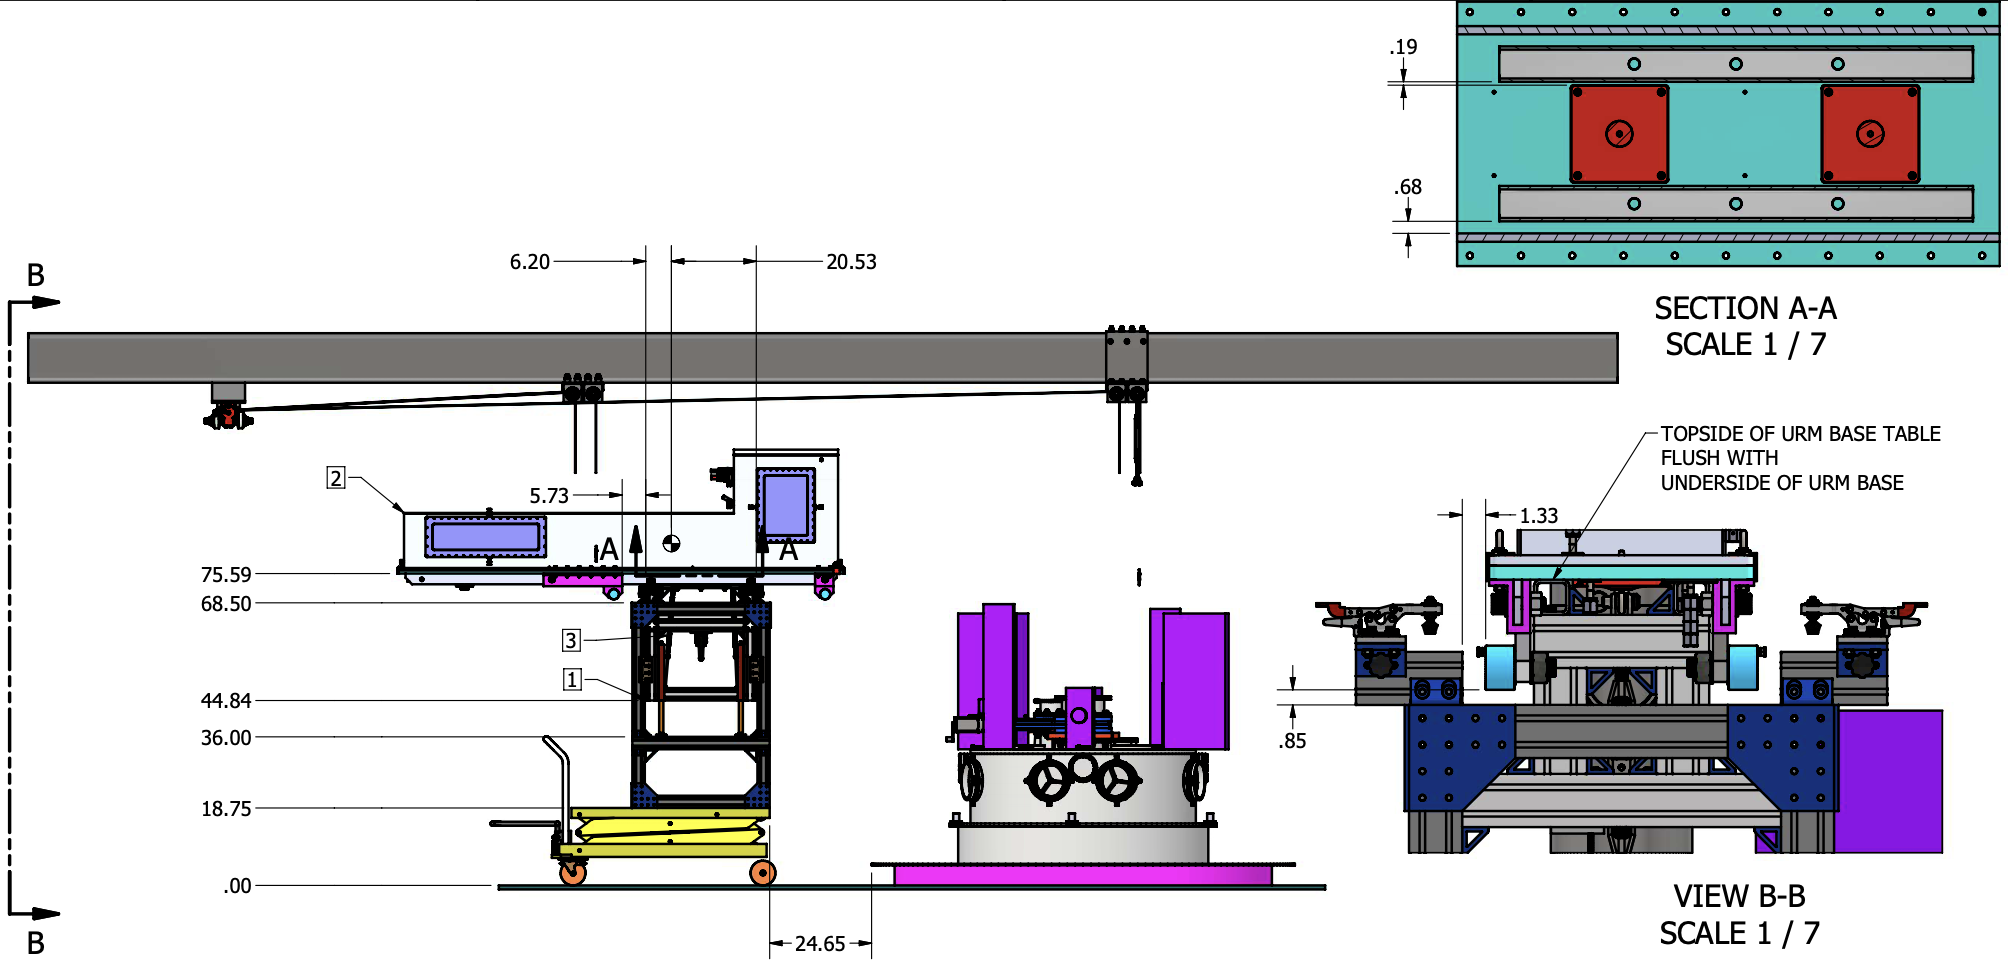
\includegraphics[width=\textwidth]{Figures/URMSecuredPreBellowsInstall}
    \caption{URM on cart prior to bellows installation.}
    \label{fig:URMpreBellows}
  \end{subfigure}
  \begin{subfigure}{0.9\textwidth}
    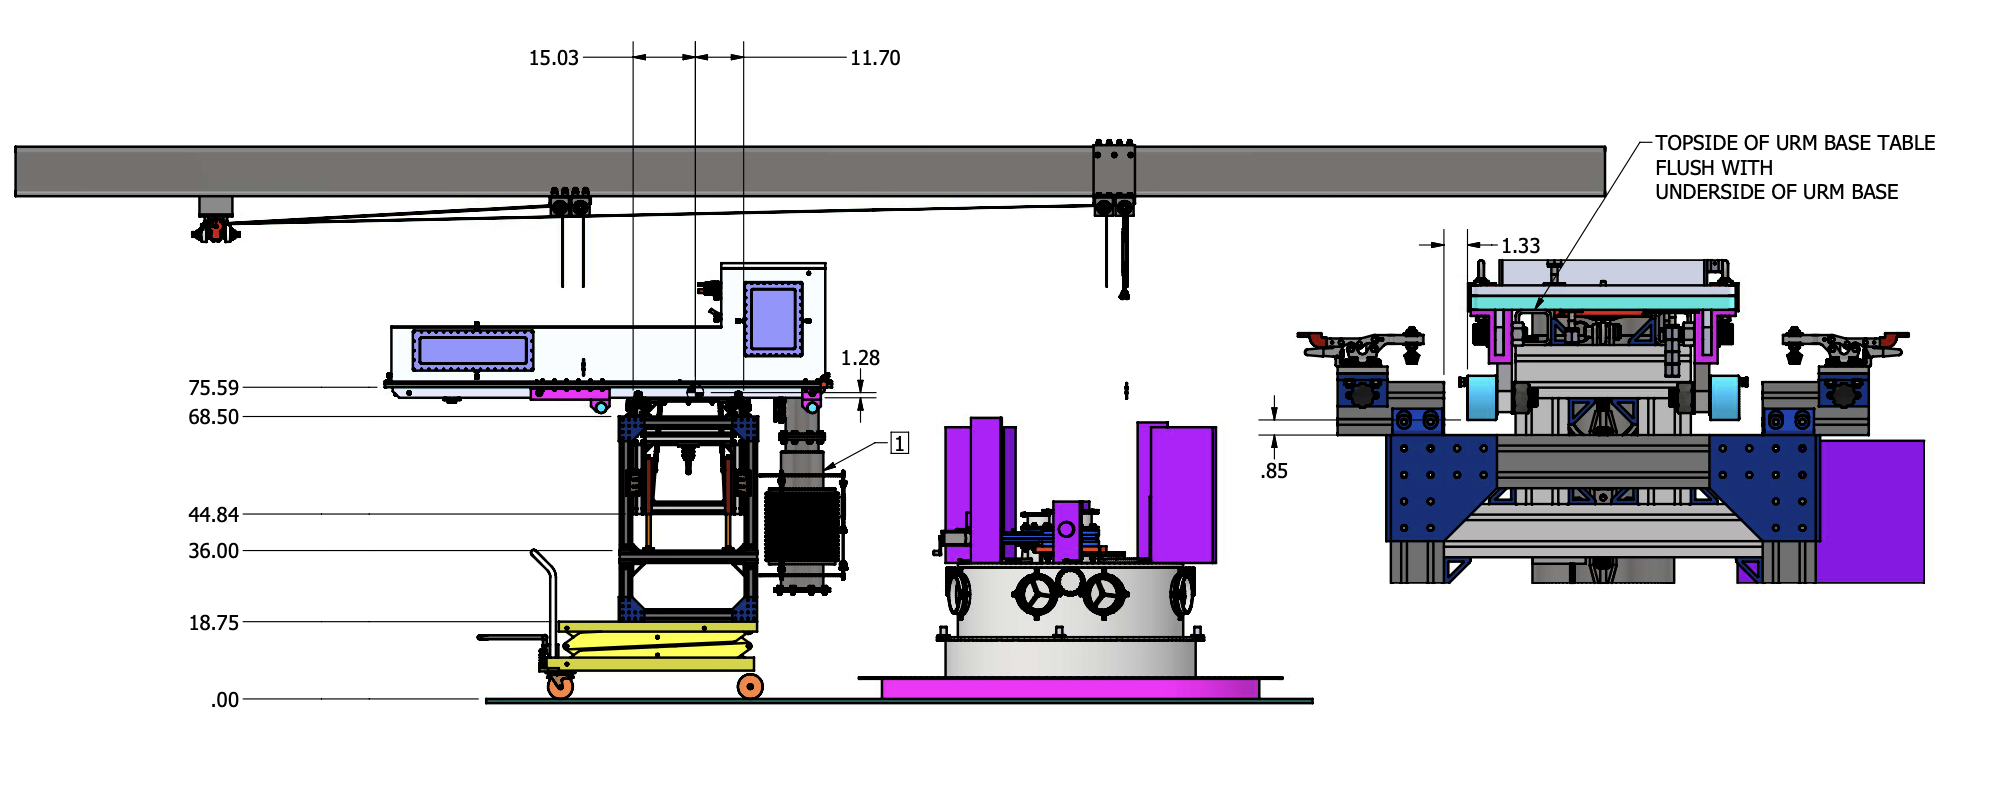
\includegraphics[width=\textwidth]{Figures/URMSecuredBellowsInstalled}
    \caption{URM on cart with the bellows installed.}
    \label{fig:URMpostBellows}
  \end{subfigure}
  \begin{subfigure}{0.9\textwidth}
    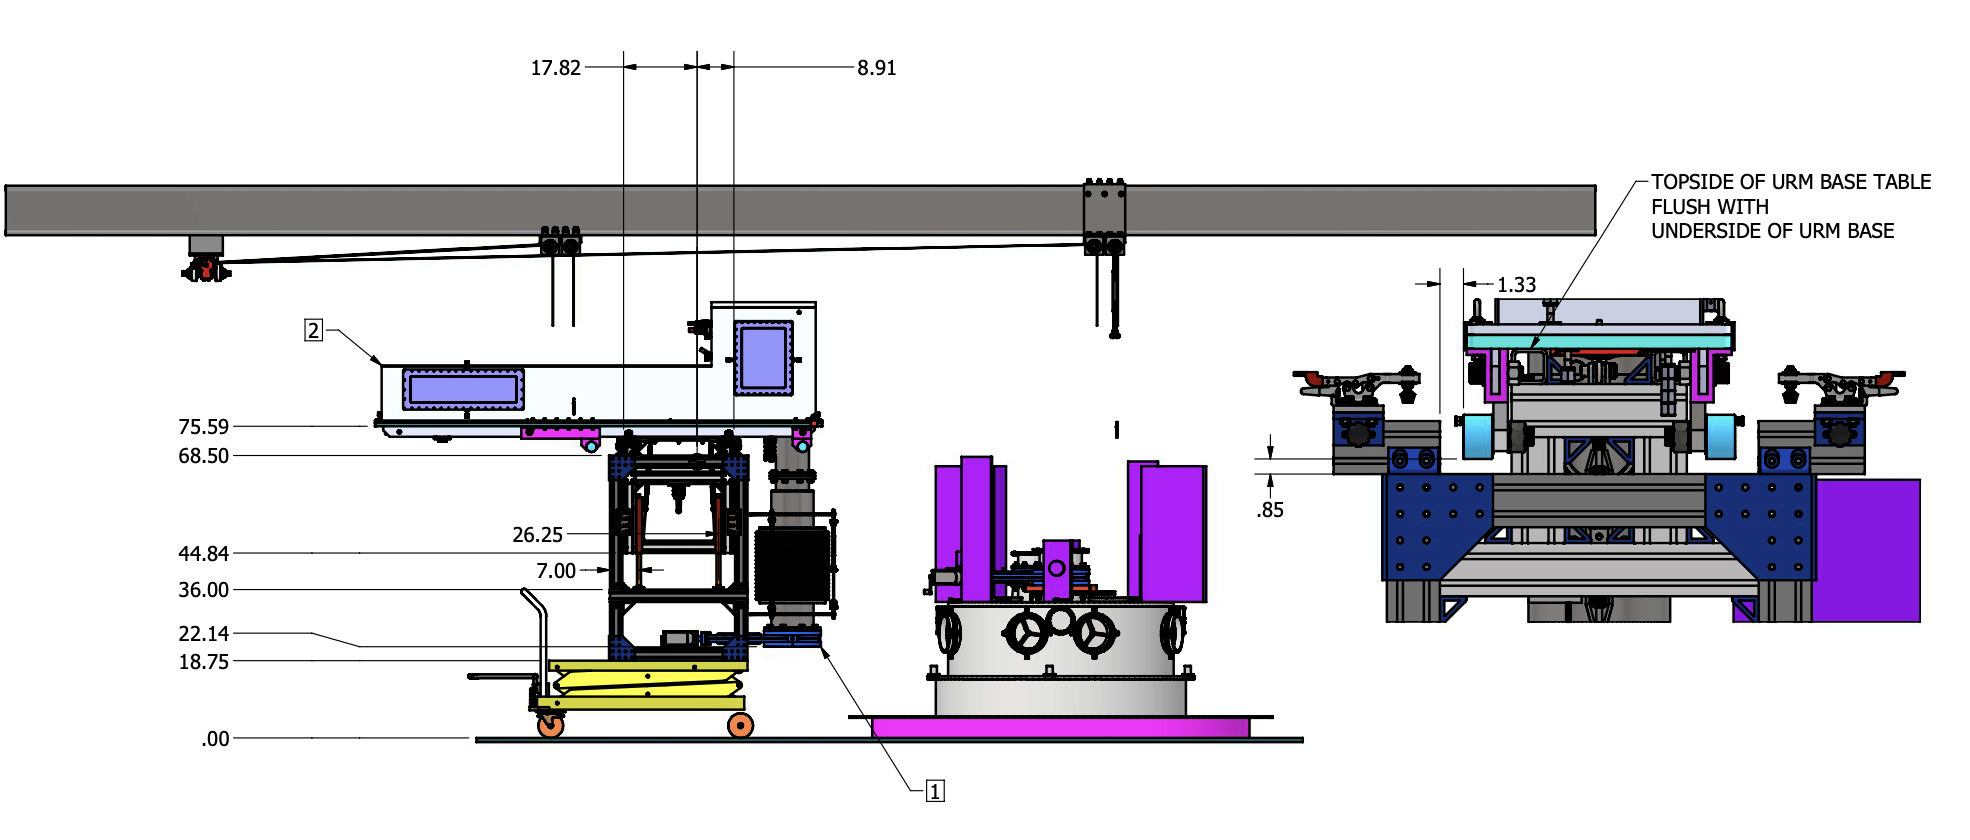
\includegraphics[width=\textwidth]{Figures/URMSecuredGateValveInstalled}
    \caption{URM on cart with gate valve installed.}
    \label{fig:URMwithGateValve}
  \end{subfigure}
  \caption{Preparing the bellows and gate valve for use}
  \label{fig:BellowsSteps}
\end{figure}

\begin{figure}
  \begin{subfigure}{0.85\textwidth}
    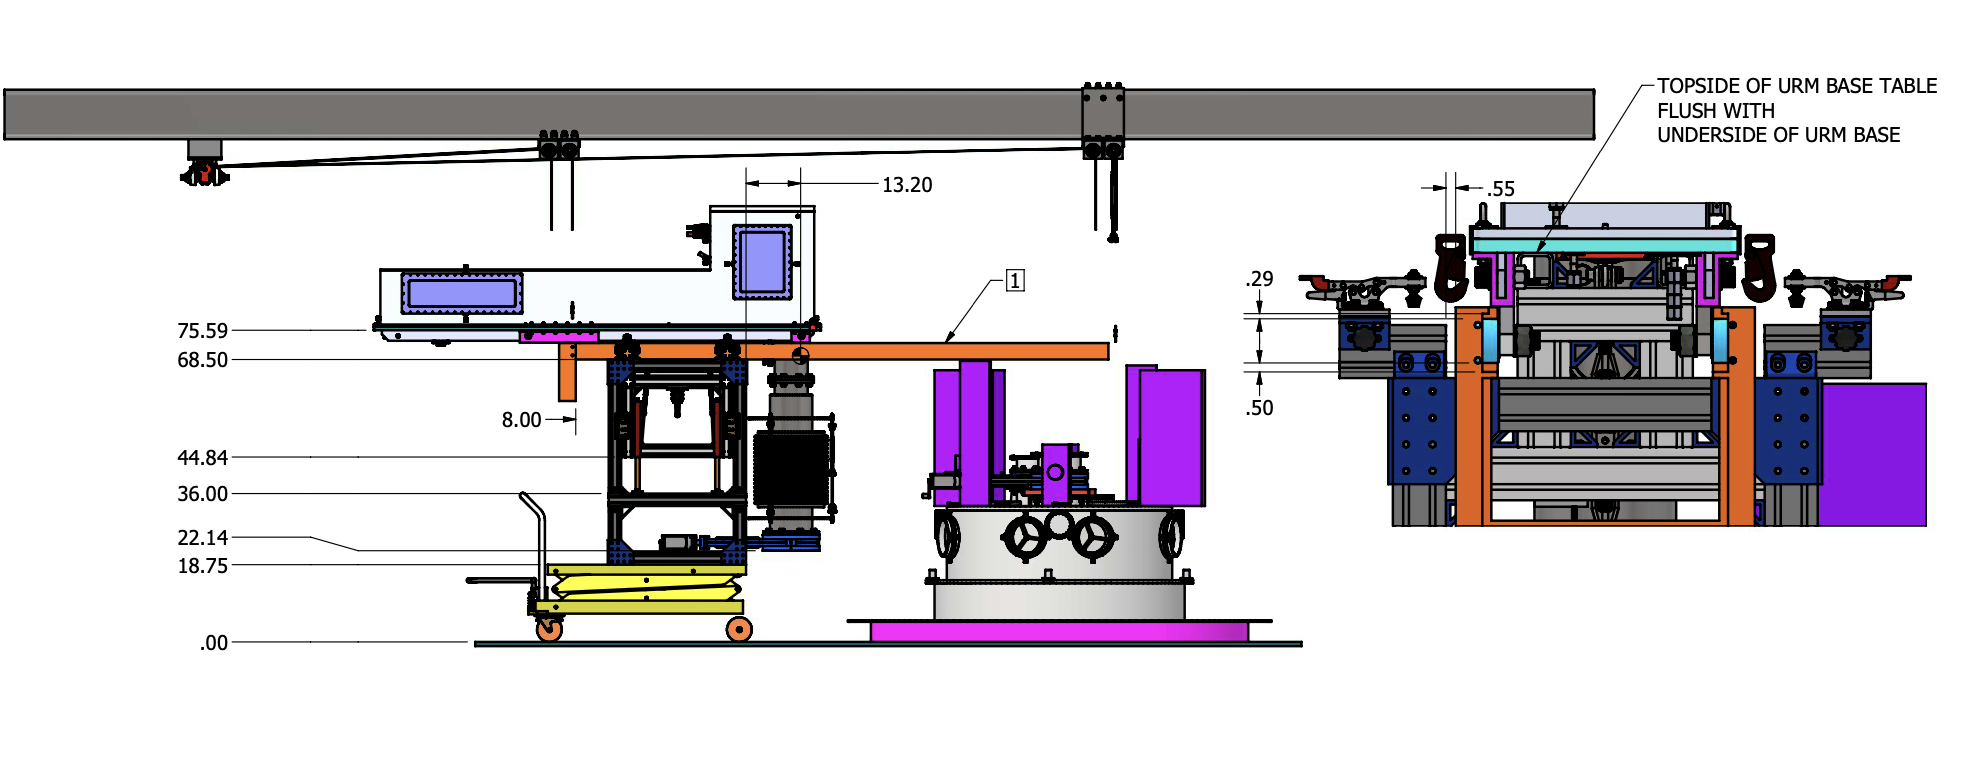
\includegraphics[width=\textwidth]{Figures/URMSecureLoadRails}
    \caption{Loading the rails onto the URM prior to lifting}
    \label{fig:URMRails}
  \end{subfigure}
  \begin{subfigure}{0.85\textwidth}
    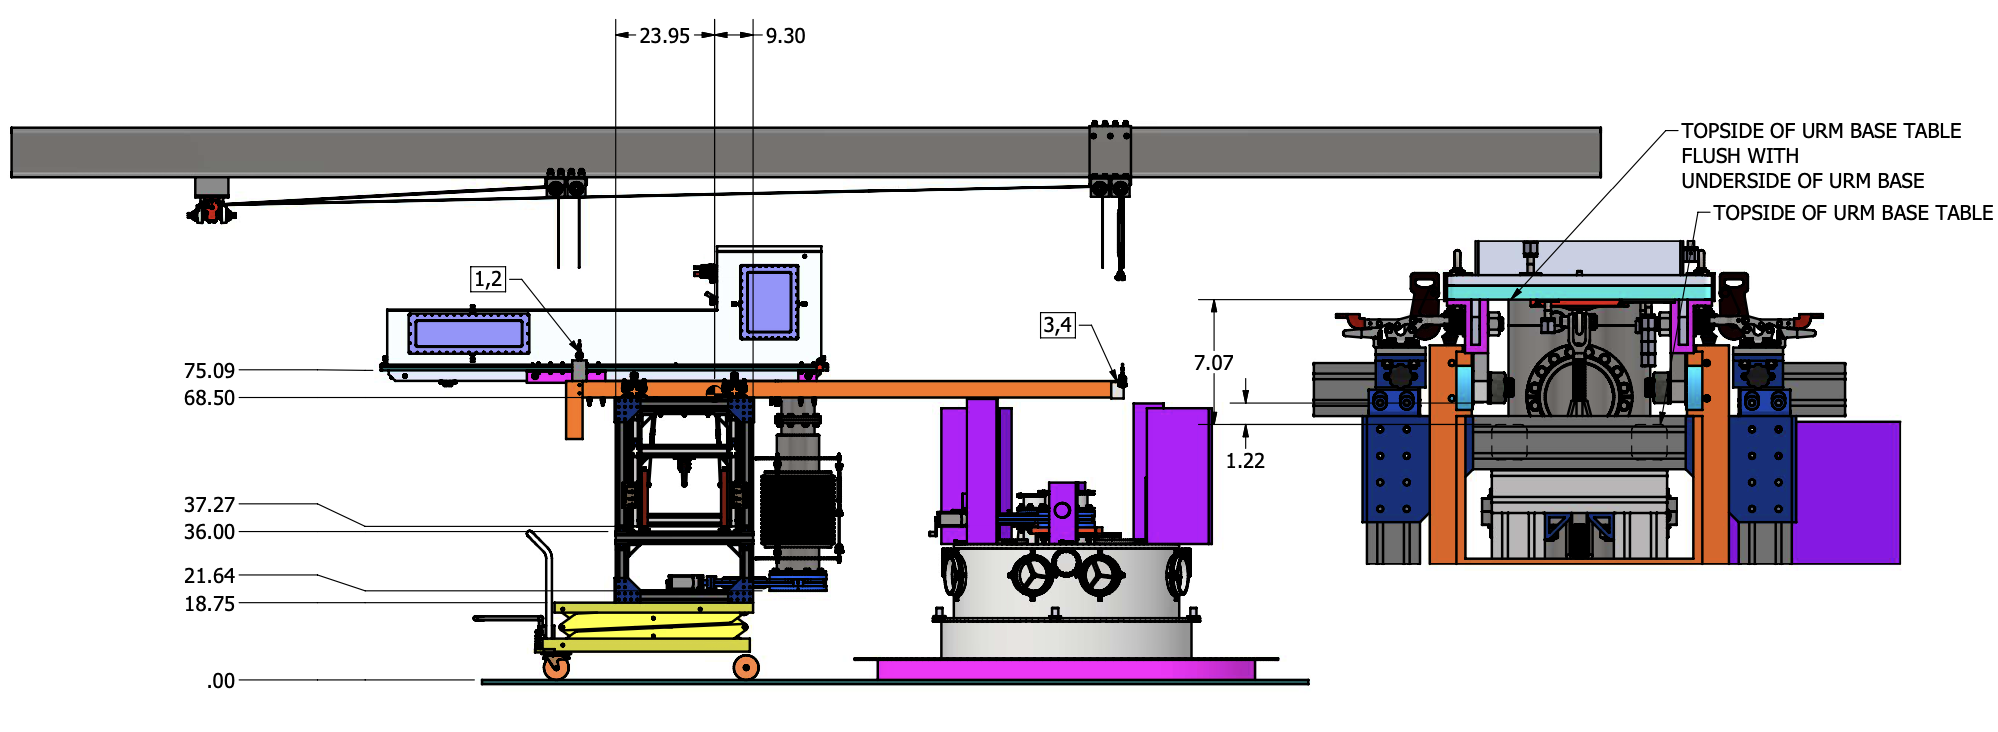
\includegraphics[width=\textwidth]{Figures/URMLoweredInstallRailHardware}
    \caption{Installing the rail front plate and rear lifting plate}
    \label{fig:URMRailHardware}
  \end{subfigure}
  \begin{subfigure}{0.85\textwidth}
    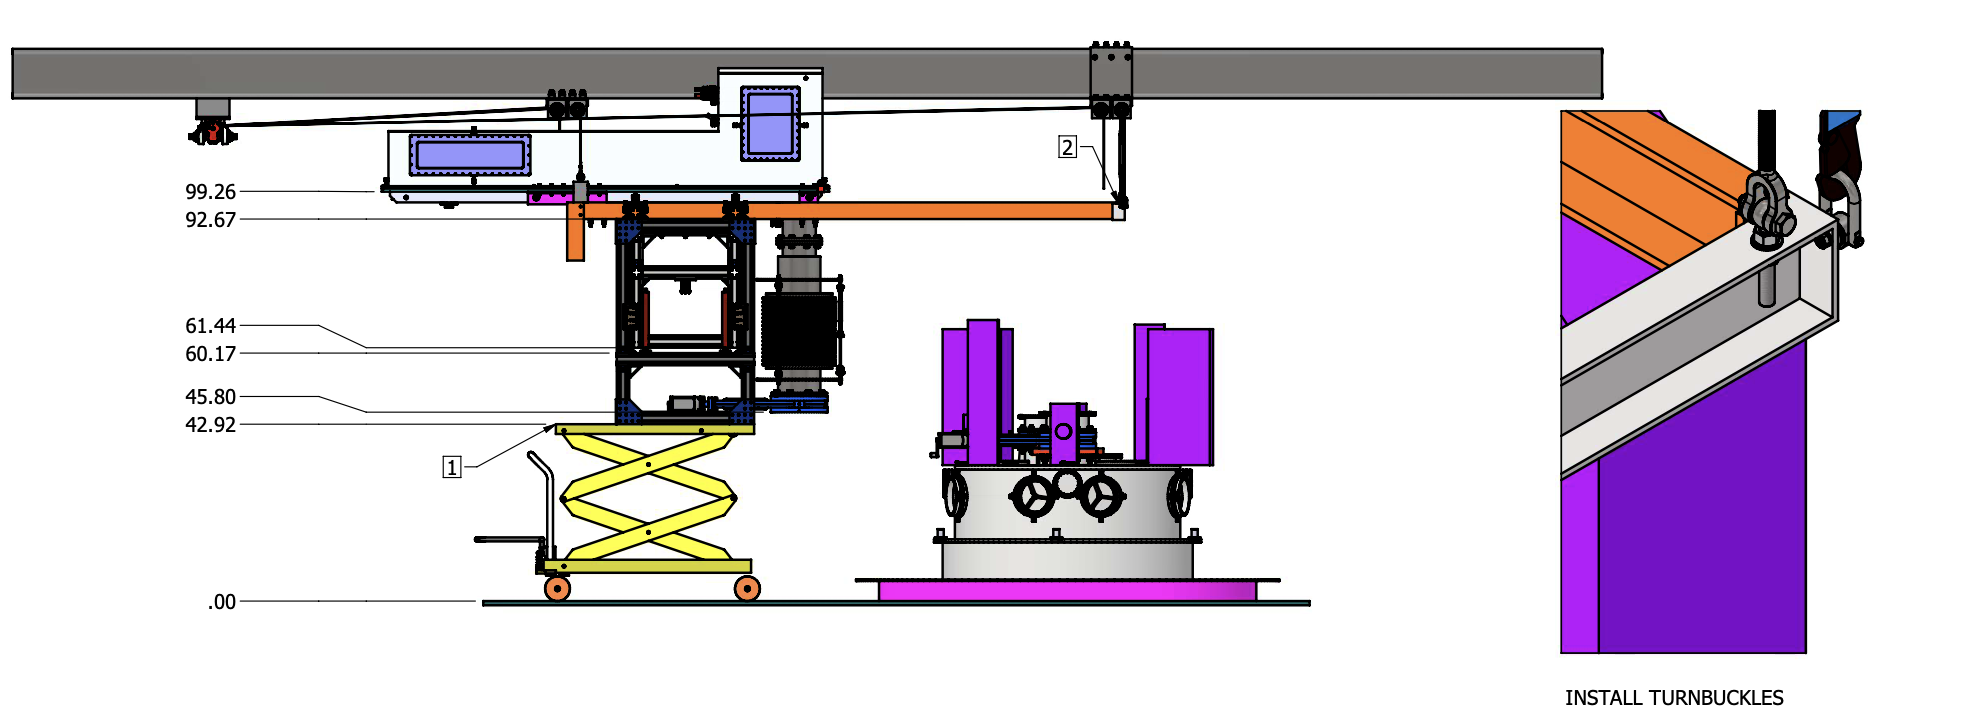
\includegraphics[width=\textwidth]{Figures/URMLiftedInstalHangers}
    \caption{Install the hangers once the URM is lifted to height}
    \label{fig:URMlifted}
  \end{subfigure}
  \begin{subfigure}{0.8\textwidth}
    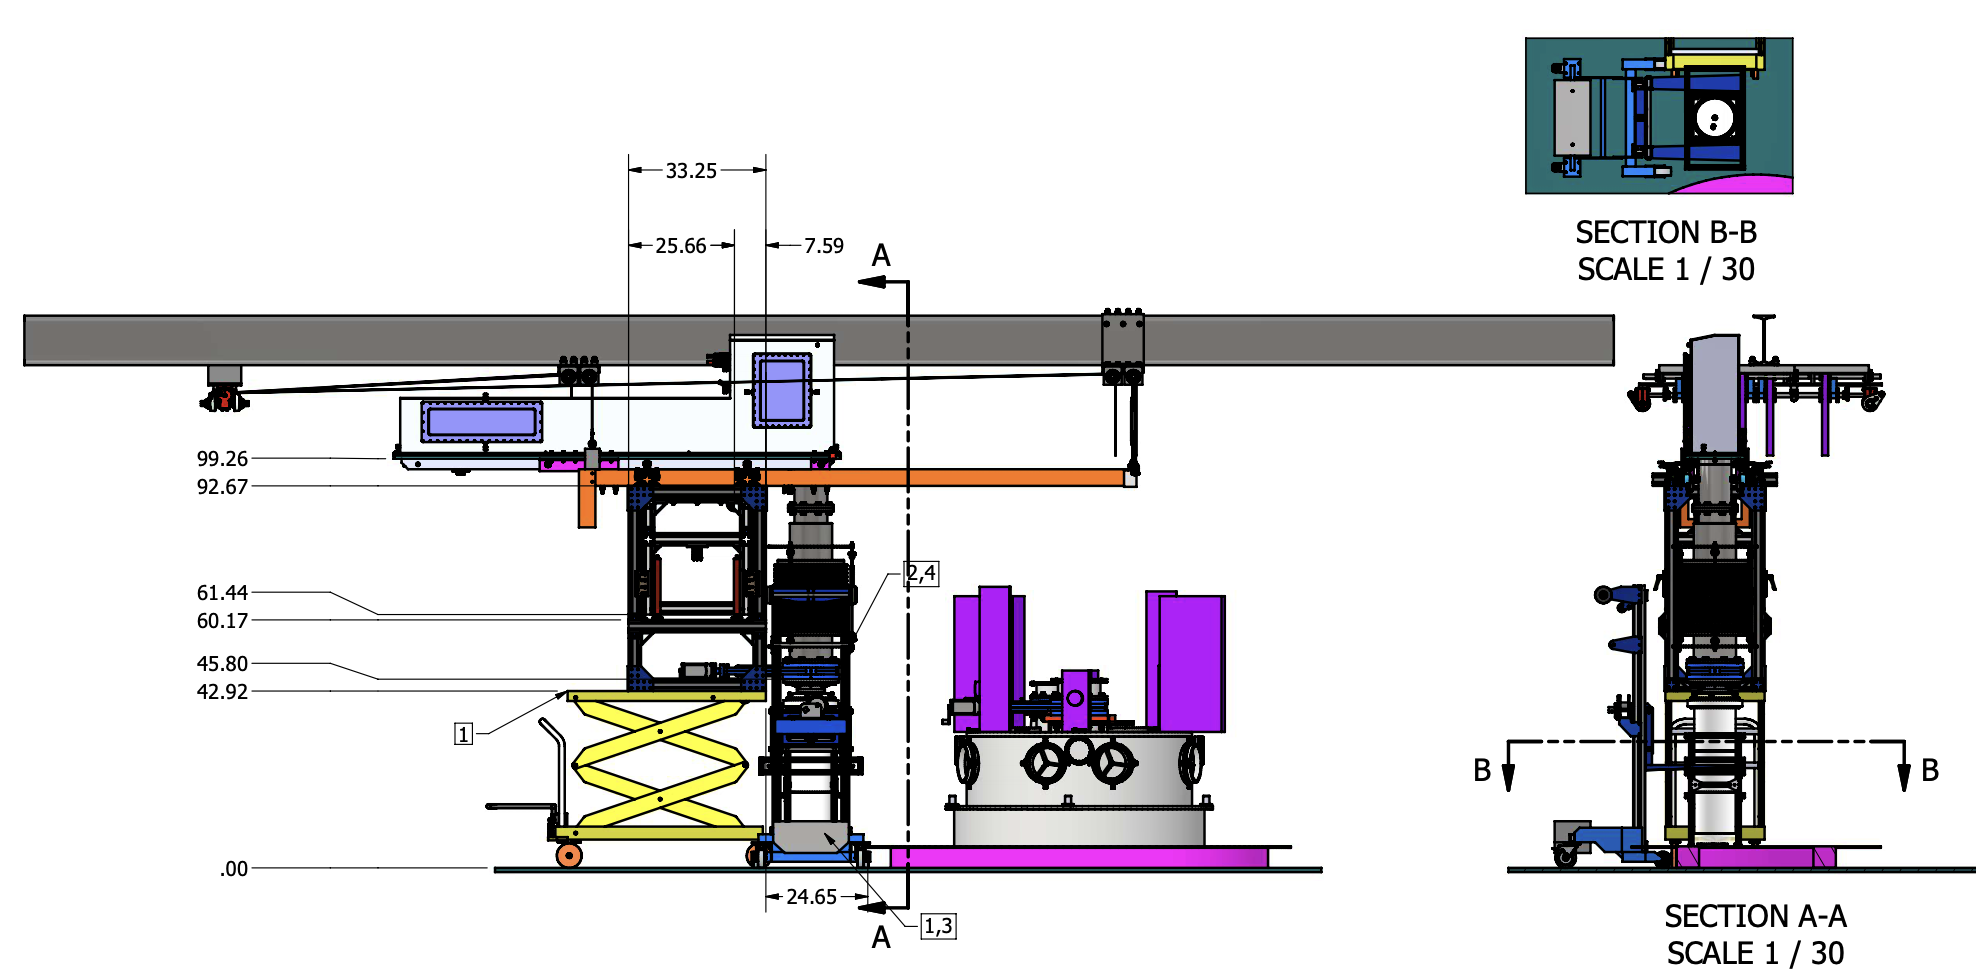
\includegraphics[width=\textwidth]{Figures/URMHungWithSCV}
    \caption{Use the source cleaning vessel with the URM at operating height.}
    \label{fig:URMSCV}
  \end{subfigure}
  \caption{Lifting the URM to Operating Height}
\end{figure}

\subsection{URM Gas Connections}\label{ss:CGConnection}
\begin{figure}
  \begin{center}
    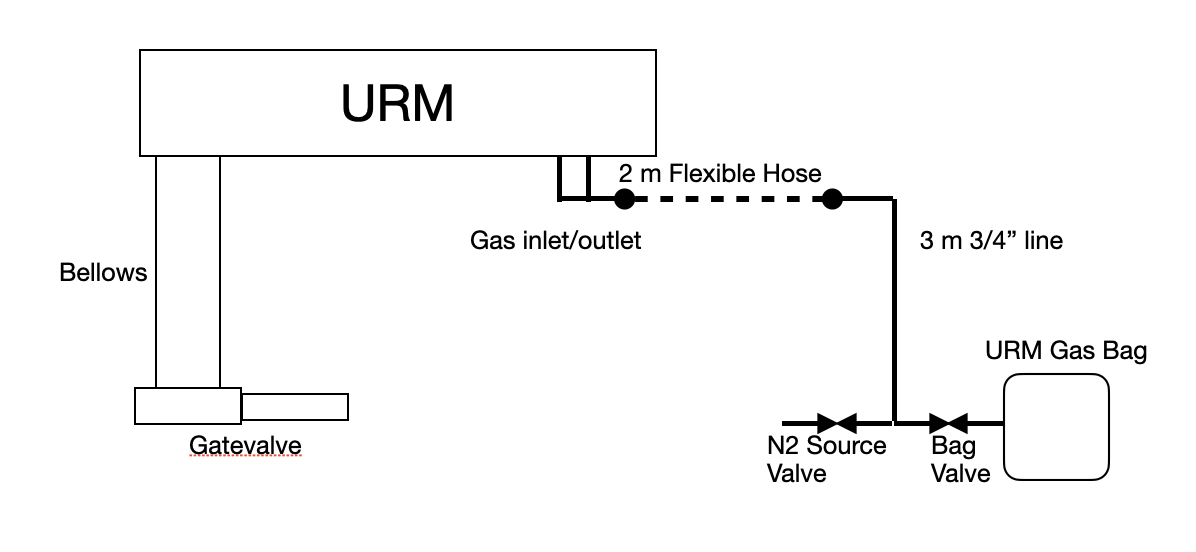
\includegraphics[width=0.8\textwidth]{URMGasFlowDiagram}
  \end{center}
  \caption{Flow diagram for the URM gas connections}
  \label{fig:URMGas}
\end{figure}

Once the umbilical, gatevalve, bellows and cover are installed on the
URM, a nitrogen atmosphere must be generated inside the URM. A 
gas bag has been constructed and suspended from a unistrut frame in
the DCR. A run of 3/4'' piping from the cover gas bag along the frame,
up the DCR North wall and across the ceiling to the DCR I-beam is meant
to provide a path between the cover gas bag and the URM. At present
this is terminated with a valve, but a flexible, stainless steel
braided hose was acquired to provide a flexible connection between the
URM and the cover gas system. A tee junction has been installed to
allow the gas to be transferred using both the end of the stretcher box
and the top of the motor box. At the cover-gas bag end, a path has been
installed to allow a path to be set to a nitrogen for the case when the
URM is open at the bottom of the source bellows with the cover gas bag
isolated. The operational cases are
\begin{enumerate}
\item URM standing alone (off UI)
  \begin{answerlist}
  \item Nitrogen source valve closed
  \item Gate valve closed
  \item Bag to URM path valve open
  \end{answerlist}
\item URM flushing (off UI)
  \begin{answerlist}
  \item Nitrogen source valve open
  \item Nitrogen source connected and supplying gas
  \item URM Gate valve open
  \item Bag to URM path valve closed
  \end{answerlist}
\item URM connected to UI before deployment
  \begin{answerlist}
  \item Bag-to-URM path valve open
  \item Nitrogen source valve closed
  \item URM Gate valve closed on top of nipple assembly
  \item UI gate valve closed
  \end{answerlist}
\item Pump-purge the nipple assembly before deployment
  \begin{answerlist}
  \item Bag-to-URM path valve open
  \item Nitrogen source valve closed
  \item Nitrogen source connected to pump purge board
  \item URM gate valve closed
  \item Pump purge board input and extraction lines connected to nipple assembly
  \item UI gate valve closed
  \item To run the pump purge procedure on the nipple assembly volume between the gate valves before they are opened;
    \begin{enumerate}[label={$\square$}]
    \item Take note of the pressure on the board gauge for the nipple assembly
    \item Double check that the gate valve state indicators are consistent with the gate valve being closed.
    \item Open a VNC instance into a DeltaV computer to monitor the UI dp.
    \item Pump out the nipple assembly at 5 L/min for 5
      minutes. Continue monitoring the UI dp to check for anomalies
      and stop if there is an unexpected drop in pressure. Resume if
      the change is determined to be unrelated to the pumping
      procedure.
    \item Switch the board to purge the nipple assembly using the
      internal solenoid valve
    \item Add nitrogen until the nipple assemblies pressure returns to
      its initial value. Continue monitoring the UI dp for pressure excursion
    \item Repeat 3 times
    \end{enumerate}
  \end{answerlist}
\item Deploying the source after pump-purge is complete
  \begin{answerlist}
  \item Bag-to-URM path valve open
  \item Nitrogen source valve closed
  \item Pump-purge board disconnected
  \item Note the UI to Deck differential pressure on Delta
  \item Open the URM gate valve
  \item Open the UI gate valve a crack and monitor the UI to Deck differential pressure on Delta
  \item If there is no variation in the pressure outside of operating limits open the gate valve completely.
  \item If there is a variation close both of the gate valves and carefully determine why the variation occurred. Further review will be necessary. 
  \item Once the gate valve is open it is expected that variations in mine pressure can be handled by the combination of the URM cover-gas and UI cover gas bags.
  \end{answerlist}
\end{enumerate}

\subsection{Field Testing the URM}\label{ss:Testing}
An important activity prior to deploying the source is to deploy a test mass in the AV to ensure that the systems can work in concert properly. For this test it is assumed that;
\begin{itemize}[label={$\square$}]
\item The umbilical and rope are loaded with the source connector attached to the end of the umbilical
\item The cover is on the URM.
\item The gate valve and bellows have been installed
\item The URM lifting system is working and complete.
\item The URM is secured to the lifting cart. 
\item The nitrogen atmosphere in the URM has been in place for a period not less than two weeks (i.e. four or more radon half lives.)
\item The source connector, with an appropriate blanking plate and weight, has undergone cleaning in the source cleaning vessel.
\end{itemize}

\begin{figure}
  \begin{subfigure}{0.9\textwidth}
    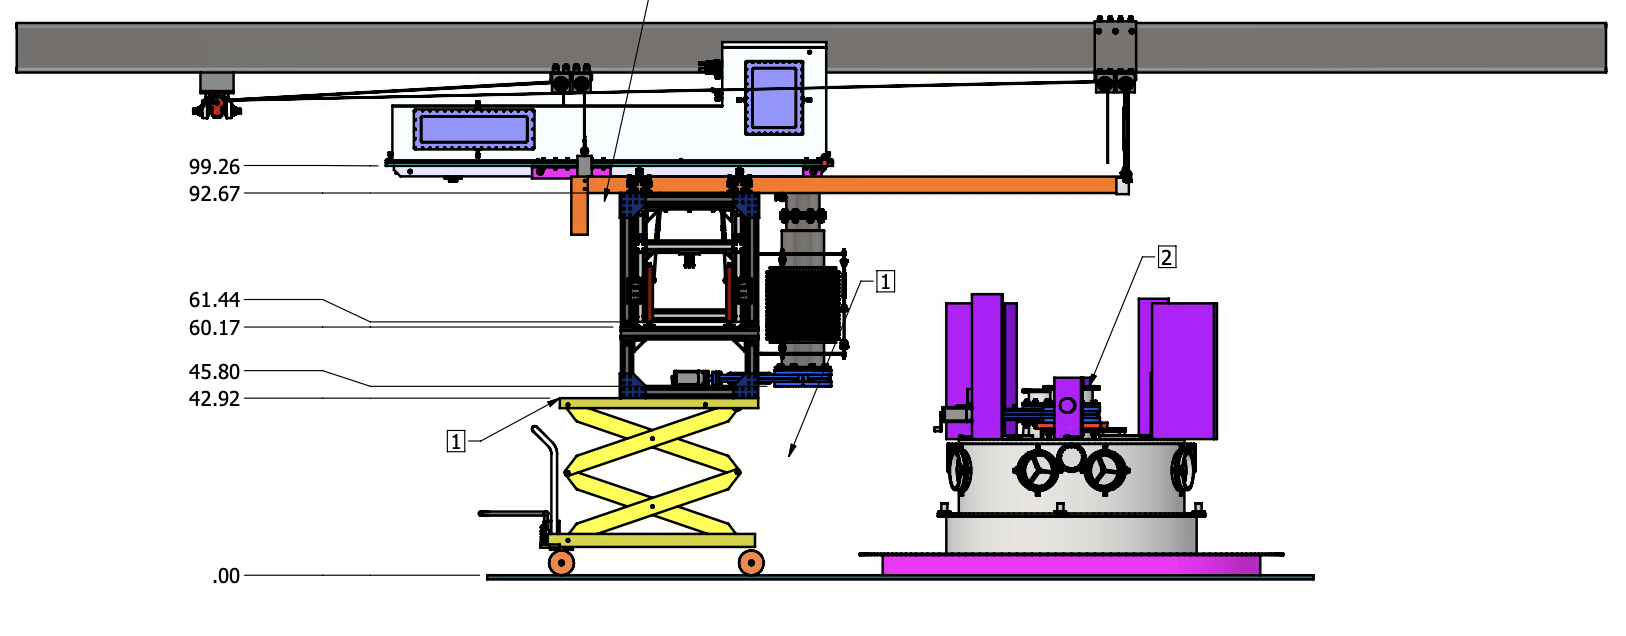
\includegraphics[width=\textwidth]{Figures/URMPreUIConnection}
    \caption{URM prior to connection with the UI}
    \label{fig:URMpreUI}
  \end{subfigure}
  \begin{subfigure}{0.9\textwidth}
    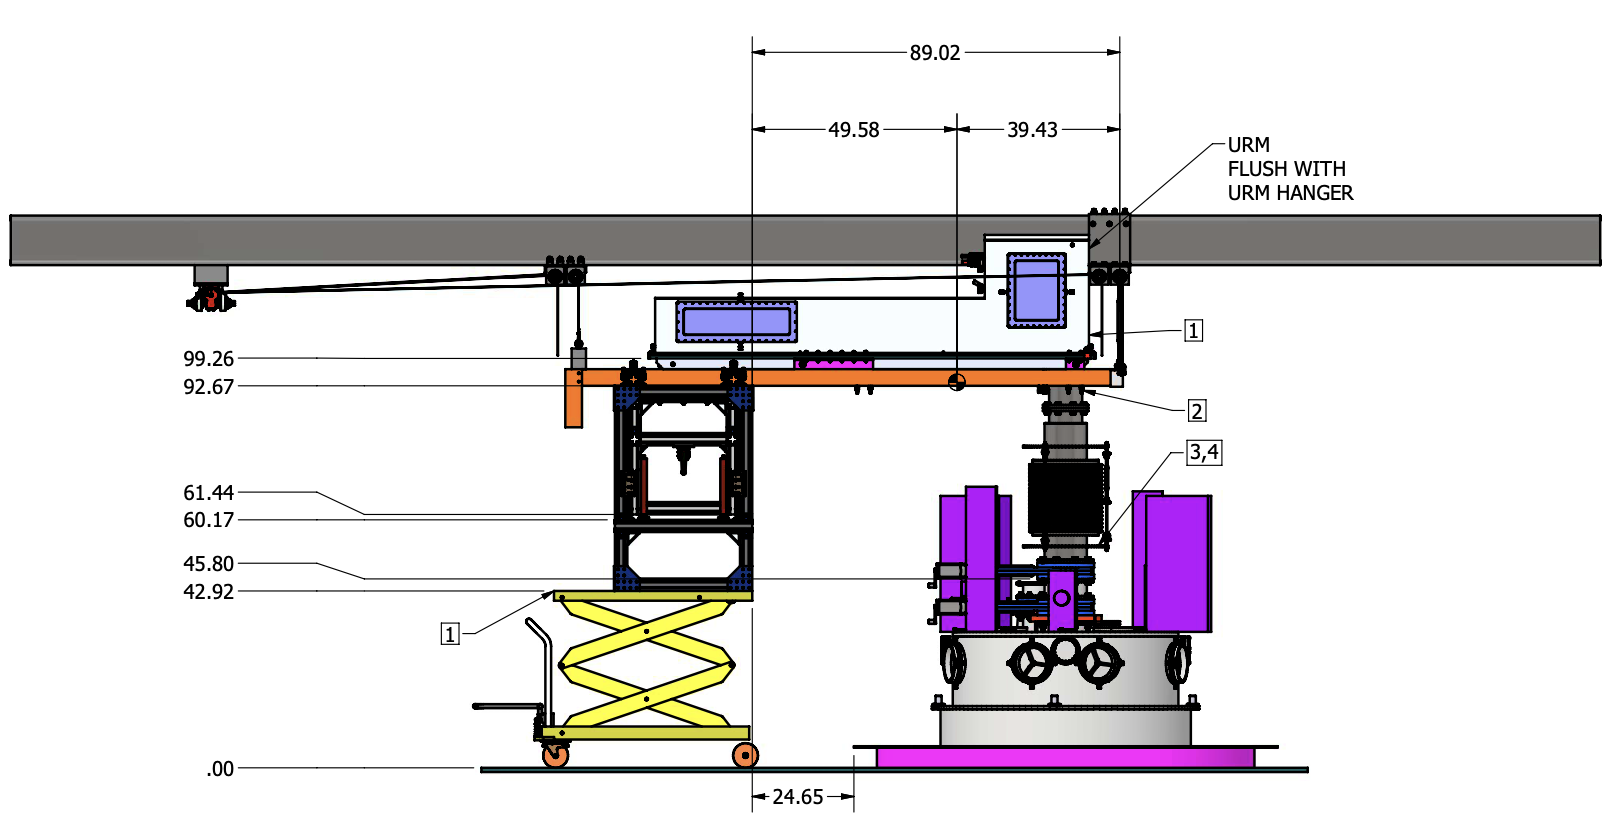
\includegraphics[width=\textwidth]{Figures/URMMountedOnUI}
    \caption{URM mounted on UI after with lifting system. Note the URM must be clamped to the rails prior to installing the gate valve.}
    \label{fig:URMpreUI}
  \end{subfigure}
  \caption{URM Deployment positions}
  \label{fig:URMDeploy}
\end{figure}

To deploy the source the operators must follow the engineer approved lifting and hanging procedure as follows;
\begin{answerlist}
\item Align the URM with the South side URM lifting path.
\item Ensure that the URM is chained to the inner table on the lifting cart
\item Mount the rails onto the URM. This is done by
  \begin{itemize}[label={$\square$}]
  \item Raising the inner table of the lifting cart to its maximum height by using the hydraulic crank
  \item Sliding the rails onto the URM wheels with the U bend of the rails on the stretcher box side of the URM.
  \item Bolt the rail front plate onto the rails using the 1/2'' bolts provided.
  \item Lower the URM so that it is supported on the rails by its wheels by turning the crank counter clockwise. Lock the inner table to the outer table using the eight yellow levers.
  \item Clamp the rails onto the lifting cart with the four side clamps.
  \end{itemize}
\item Raise the URM gatevalve so that it is no longer resting on the cart table through the use of the bellows turnbuckles. 
\item Connect the rails to the lifting mechanism straps using the available eye-bolts on the front and back of the URM.
\item With one person on the winch and a second on the cart, lift the URM to operating height. Most of the effort is from the lifting cart; there should never be slack on the winch straps but never so much that it takes all of the URM weight.
\item With the URM at operating height, install the turnbuckles installed on the hangers to fix the URM rails into position. Set the safety stop bars in place at the base of the table.
\item Undo the turnbuckles chaining the URM to the cart. Unlock the inner table and lower it until it is flush with the surface of the outer table.
\item Remove the cover from the 10 inch gatevalve nipple assembly and check that the requisite o-rings are in place.
\item Push the URM into position over the UI.
\item Ensure that the gatevalve is aligned with the nipple assembly on the 10 inch gate valve
\item Clamp the URM into position on the rails so that the URM can no longer roll freely
\item Slowly lower the gatevalve onto the nipple assembly using the bellows turnbuckles. It is essential that the gatevalve lands evenly and without damaging the flanges Start threading bolts into the gatevalve as soon as they can reach.
\item Once the bellows gatevalve is supported by the nipple assembly, tighten all of the bolts in a star pattern to ensure that force is distributed evenly across the flange
\item Measure the height of the viewport on the URM source tee relative to the height of the UI by aligning the laser level with the viewport. Remove the viewport cover and align the source pivot with the laser level. Note the top of the UI is 1409.63 cm from the center of the AV; locate the source to be the measured difference between the top of the UI and the reference position in addition to 1409.63 cm.
\item Pump and purge the space inside the nipple assembly (as described in section \ref{ss:CGConnection}).
\item Open the bellows gate valve
\item Check the differential pressure between the UI and Deck using DeltaV
\item Slowly open the UI gatevalve. Actively monitor the differential pressure between the UI and Deck using DeltaV. If there is a change in the differential pressure for between the deck and the AV, close the gatevalve. Check that the cover gas bag for the URM is connected and responding to changes and that the UI cover gas bag also responding within their nominal operating range. Once those checks have been completed with the participation and approval of a cover gas expert, and all of the systems are behaving properly, resume opening the gate valves. If the safe operating pressure is maintained, proceed with opening the gatevalve fully.
\item Lower the test mass into the UI. Stop when the test mass is approximately 30 cm below the top of the UI.
\item Connect the side ropes to the source carriage. The side ropes will need to be connected to the source in the manip interface as well.
\item Lower the test mass into the AV and drive the source to various locations. Efforts should be made to test the limits of motion for the manipulator system given the test mass. Care must be taken to ensure that the drive limits are observed (tensions must remain with limits for the ropes, etc.).
\item Retrieve the test mass from the AV. Stop the test mass 30 cm below the UI top to remove the side ropes.
\item Raise the source into the bellows. Carefully close the UI gate valve. Then close the bellows gate valve.
\item Check the location of the source pivot through the viewport. Compare the source carriage height after the deployment to that value that is predicted by manip using the measurements prior to deployment. Note any changes relative to the expectation in the log book.
\end{answerlist}

\section{Scheduling}

The tasks to be completed prior to source deployment can be placed onto a matrix of weeks of work. Each week is occupied by 5 shifts worth of tasks. Some of the tasks may take less time, but the decision to advance the schedule should only be done as tasks are complete. For reference this block schedule extends beyond the procedures given here to include Laserball deployment. 
\begin{table}
  \caption{Block scheduling for the tasks remaining in the assembly of the URM}
  \begin{tabular}{|c|p{13cm}|c|}
    \hline
    Week & Task & Personnel \\
    \hline
    0 & \vspace{-0.7cm} \begin{itemize}[label={$\square$}]
    \item Preparation of umbilical feed-through plate; Sec.\ref{ss:umbPrepFeed} \end{itemize} \vspace{-0.5cm} & Machine shop \\ \hline
    1 & \vspace{-0.7cm} \begin{itemize}[label={$\square$}]
    \item Remove URM cover; Sec.\ref{ss:rmCov}
    \item Electrical systems check; Sec.\ref{ss:elecSSC} 
    \item Install umbilical feed-through plate on umbilical; Sec.\ref{ss:umbPrepFeed} 
    \item Install umbilical on URM; Sec.\ref{ss:UmbInstall}
    \item Install rope on URM; Sec. \ref{ss:RopeInstall} 
    \item Install URM cover; Sec.\ref{ss:CoverInstall} 
    \end{itemize} \vspace{-0.5cm} 
    & 4 workers \\\hline
    2 & \vspace{-0.7cm}\begin{itemize}[label={$\square$}]
    \item Electrical systems check; Sec.\ref{ss:elecSSC}
    \item Transfer URM from cart to lifting table; Sec.\ref{ss:transfer}
    \item Install source tee flange; Sec.\ref{ss:SourceTeeInstall}
    \item Final Umbilical cleaning; Sec.\ref{ss:UmbClean}
    \item Install source connector on umbilical; Sec.\ref{ss:SourceConn}
      % \item Install the wheels on the URM
    \item Install source bellows; Sec.\ref{sss:BellowsInstall}
    \item Install gate valve; Sec.\ref{sss:GateValveInstall}
    \end{itemize} \vspace{-0.5cm} 
    & 6 workers \\ \hline
    3 & \vspace{-0.7cm} \begin{itemize}[label={$\square$}]
    \item Purge the URM and connect to the cover gas system; Sec.\ref{ss:CGConnection}
    \end{itemize} \vspace{-0.5cm} 
    & 2 workers \\\hline
    4 & \vspace{-0.7cm} \begin{itemize}[label={$\square$}]
    \item Connect and clean the dummy source with source cleaning vessel
    \end{itemize} \vspace{-0.5cm} 
    & 2 workers \\\hline
    5 &  \vspace{-0.7cm} \begin{itemize}[label={$\square$}]
    \item Connect URM to UI; Sec.\ref{ss:CGConnection}
    \item Field test the manipulator system.; Sec.\ref{ss:Testing}
    \end{itemize} \vspace{-0.5cm} 
    & 3 workers \\
    6 & \vspace{-0.7cm} \begin{itemize}[label={$\square$}]
    \item Disconnect URM from UI
    \item Disconnect dummy source and connect Laserball to URM
    \item Clean Laserball source with source cleaning vessel
    \item Prepare/optimize Dye-laser for use
    \end{itemize} \vspace{-0.5cm} 
    & 3 workers \\ \hline
    7 & \vspace{-0.7cm} \begin{itemize}[label={$\square$}]
    \item Run Laserball deployment program
    \end{itemize} \vspace{-0.5cm} 
    & 4-6 workers \\\hline
  \end{tabular}
  \label{tab:blockSchedule}
\end{table}

% It is expected that the earliest that the pre-requisites can be fulfilled is the third week of 2025 (week of January 13). This places the end of week 5 as February 14 2025. Thus the Laserball installation and cleaning can take place the following week, starting February 18, with a potential deployment the week of February 24. 

\end{document}
